\documentclass[a4paper]{article}

\def\npart {III}
\def\nterm {Lent}
\def\nyear {2017}
\def\nlecturer {A. G. Kovalev}
\def\ncourse {Riemannian Geometry}
\def\nlectures {TTS.12}

% Imports
\ifx \nextra \undefined
  \usepackage[pdftex,
    hidelinks,
    pdfauthor={Dexter Chua},
    pdfsubject={Cambridge Maths Notes: Part \npart\ - \ncourse},
    pdftitle={Part \npart\ - \ncourse},
  pdfkeywords={Cambridge Mathematics Maths Math \npart\ \nterm\ \nyear\ \ncourse}]{hyperref}
  \title{Part \npart\ - \ncourse}
\else
  \usepackage[pdftex,
    hidelinks,
    pdfauthor={Dexter Chua},
    pdfsubject={Cambridge Maths Notes: Part \npart\ - \ncourse\ (\nextra)},
    pdftitle={Part \npart\ - \ncourse\ (\nextra)},
  pdfkeywords={Cambridge Mathematics Maths Math \npart\ \nterm\ \nyear\ \ncourse\ \nextra}]{hyperref}

  \title{Part \npart\ - \ncourse \\ {\Large \nextra}}
\fi

\author{Lectured by \nlecturer \\\small Notes taken by Dexter Chua}
\date{\nterm\ \nyear}

\usepackage{alltt}
\usepackage{amsfonts}
\usepackage{amsmath}
\usepackage{amssymb}
\usepackage{amsthm}
\usepackage{booktabs}
\usepackage{caption}
\usepackage{enumitem}
\usepackage{fancyhdr}
\usepackage{graphicx}
\usepackage{mathtools}
\usepackage{microtype}
\usepackage{multirow}
\usepackage{pdflscape}
\usepackage{pgfplots}
\usepackage{siunitx}
\usepackage{tabularx}
\usepackage{tikz}
\usepackage{tkz-euclide}
\usepackage[normalem]{ulem}
\usepackage[all]{xy}

\pgfplotsset{compat=1.12}

\pagestyle{fancyplain}
\lhead{\emph{\nouppercase{\leftmark}}}
\ifx \nextra \undefined
  \rhead{
    \ifnum\thepage=1
    \else
      \npart\ \ncourse
    \fi}
\else
  \rhead{
    \ifnum\thepage=1
    \else
      \npart\ \ncourse\ (\nextra)
    \fi}
\fi
\usetikzlibrary{arrows}
\usetikzlibrary{decorations.markings}
\usetikzlibrary{decorations.pathmorphing}
\usetikzlibrary{positioning}
\usetikzlibrary{fadings}
\usetikzlibrary{intersections}
\usetikzlibrary{cd}

\newcommand*{\Cdot}{\raisebox{-0.25ex}{\scalebox{1.5}{$\cdot$}}}
\newcommand {\pd}[2][ ]{
  \ifx #1 { }
    \frac{\partial}{\partial #2}
  \else
    \frac{\partial^{#1}}{\partial #2^{#1}}
  \fi
}

% Theorems
\theoremstyle{definition}
\newtheorem*{aim}{Aim}
\newtheorem*{axiom}{Axiom}
\newtheorem*{claim}{Claim}
\newtheorem*{cor}{Corollary}
\newtheorem*{defi}{Definition}
\newtheorem*{eg}{Example}
\newtheorem*{fact}{Fact}
\newtheorem*{law}{Law}
\newtheorem*{lemma}{Lemma}
\newtheorem*{notation}{Notation}
\newtheorem*{prop}{Proposition}
\newtheorem*{thm}{Theorem}

\renewcommand{\labelitemi}{--}
\renewcommand{\labelitemii}{$\circ$}
\renewcommand{\labelenumi}{(\roman{*})}

\let\stdsection\section
\renewcommand\section{\newpage\stdsection}

% Strike through
\def\st{\bgroup \ULdepth=-.55ex \ULset}

% Maths symbols
\newcommand{\bra}{\langle}
\newcommand{\ket}{\rangle}

\newcommand{\N}{\mathbb{N}}
\newcommand{\Z}{\mathbb{Z}}
\newcommand{\Q}{\mathbb{Q}}
\renewcommand{\H}{\mathbb{H}}
\newcommand{\R}{\mathbb{R}}
\newcommand{\C}{\mathbb{C}}
\newcommand{\Prob}{\mathbb{P}}
\renewcommand{\P}{\mathbb{P}}
\newcommand{\E}{\mathbb{E}}
\newcommand{\F}{\mathbb{F}}
\newcommand{\cU}{\mathcal{U}}
\newcommand{\RP}{\mathbb{RP}}
\newcommand{\CP}{\mathbb{CP}}

\newcommand{\ph}{\,\cdot\,}

\DeclareMathOperator{\sech}{sech}
\DeclareMathOperator{\cosech}{cosech}
\DeclareMathOperator{\cosec}{cosec}

\DeclareMathOperator{\covol}{covol}
\DeclareMathOperator{\vol}{vol}

\let\Im\relax
\let\Re\relax
\DeclareMathOperator{\Im}{Im}
\DeclareMathOperator{\Re}{Re}
\DeclareMathOperator{\im}{im}
\DeclareMathOperator{\image}{image}
\DeclareMathOperator{\Ann}{Ann}

\DeclareMathOperator*{\res}{res}
\DeclareMathOperator{\Res}{Res}
\DeclareMathOperator{\Ind}{Ind}

\DeclareMathOperator{\tr}{tr}
\DeclareMathOperator{\diag}{diag}
\DeclareMathOperator{\rank}{rank}
\DeclareMathOperator{\card}{card}
\DeclareMathOperator{\spn}{span}
\DeclareMathOperator{\adj}{adj}

\DeclareMathOperator{\erf}{erf}
\DeclareMathOperator{\erfc}{erfc}

\DeclareMathOperator{\ord}{ord}
\DeclareMathOperator{\Sym}{Sym}

\DeclareMathOperator{\sgn}{sgn}
\DeclareMathOperator{\orb}{orb}
\DeclareMathOperator{\stab}{stab}
\DeclareMathOperator{\ccl}{ccl}

\DeclareMathOperator{\lcm}{lcm}
\DeclareMathOperator{\hcf}{hcf}

\DeclareMathOperator{\Int}{Int}
\DeclareMathOperator{\id}{id}

\DeclareMathOperator{\betaD}{beta}
\DeclareMathOperator{\gammaD}{gamma}
\DeclareMathOperator{\Poisson}{Poisson}
\DeclareMathOperator{\binomial}{binomial}
\DeclareMathOperator{\multinomial}{multinomial}
\DeclareMathOperator{\Bernoulli}{Bernoulli}
\DeclareMathOperator{\like}{like}

\DeclareMathOperator{\var}{var}
\DeclareMathOperator{\cov}{cov}
\DeclareMathOperator{\bias}{bias}
\DeclareMathOperator{\mse}{mse}
\DeclareMathOperator{\corr}{corr}

\DeclareMathOperator{\otp}{otp}
\DeclareMathOperator{\dom}{dom}

\DeclareMathOperator{\Root}{Root}
\DeclareMathOperator{\supp}{supp}
\DeclareMathOperator{\rel}{rel}
\DeclareMathOperator{\Hom}{Hom}
\DeclareMathOperator{\Aut}{Aut}
\DeclareMathOperator{\Gal}{Gal}
\DeclareMathOperator{\Mat}{Mat}
\DeclareMathOperator{\End}{End}
\DeclareMathOperator{\Char}{char}
\DeclareMathOperator{\ev}{ev}
\DeclareMathOperator{\St}{St}
\DeclareMathOperator{\Lk}{Lk}
\DeclareMathOperator{\disc}{disc}
\DeclareMathOperator{\Isom}{Isom}
\DeclareMathOperator{\length}{length}
\DeclareMathOperator{\energy}{energy}
\DeclareMathOperator{\area}{area}
\DeclareMathOperator{\Syl}{Syl}
\DeclareMathOperator{\cl}{cl}
\DeclareMathOperator{\fix}{fix}

\newcommand{\GL}{\mathrm{GL}}
\newcommand{\SL}{\mathrm{SL}}
\newcommand{\PGL}{\mathrm{PGL}}
\newcommand{\PSL}{\mathrm{PSL}}
\newcommand{\PSU}{\mathrm{PSU}}
\newcommand{\Or}{\mathrm{O}}
\newcommand{\SO}{\mathrm{SO}}
\newcommand{\U}{\mathrm{U}}
\newcommand{\SU}{\mathrm{SU}}

\renewcommand{\d}{\mathrm{d}}
\newcommand{\D}{\mathrm{D}}

\tikzset{->/.style = {decoration={markings,
                                  mark=at position 1 with {\arrow[scale=2]{latex'}}},
                      postaction={decorate}}}
\tikzset{<-/.style = {decoration={markings,
                                  mark=at position 0 with {\arrowreversed[scale=2]{latex'}}},
                      postaction={decorate}}}
\tikzset{<->/.style = {decoration={markings,
                                   mark=at position 0 with {\arrowreversed[scale=2]{latex'}},
                                   mark=at position 1 with {\arrow[scale=2]{latex'}}},
                       postaction={decorate}}}
\tikzset{->-/.style = {decoration={markings,
                                   mark=at position #1 with {\arrow[scale=2]{latex'}}},
                       postaction={decorate}}}
\tikzset{-<-/.style = {decoration={markings,
                                   mark=at position #1 with {\arrowreversed[scale=2]{latex'}}},
                       postaction={decorate}}}

\tikzset{circ/.style = {fill, circle, inner sep = 0, minimum size = 3}}
\tikzset{mstate/.style={circle, draw, blue, text=black, minimum width=0.7cm}}

\definecolor{mblue}{rgb}{0.2, 0.3, 0.8}
\definecolor{morange}{rgb}{1, 0.5, 0}
\definecolor{mgreen}{rgb}{0.1, 0.4, 0.2}
\definecolor{mred}{rgb}{0.5, 0, 0}

\def\drawcirculararc(#1,#2)(#3,#4)(#5,#6){%
    \pgfmathsetmacro\cA{(#1*#1+#2*#2-#3*#3-#4*#4)/2}%
    \pgfmathsetmacro\cB{(#1*#1+#2*#2-#5*#5-#6*#6)/2}%
    \pgfmathsetmacro\cy{(\cB*(#1-#3)-\cA*(#1-#5))/%
                        ((#2-#6)*(#1-#3)-(#2-#4)*(#1-#5))}%
    \pgfmathsetmacro\cx{(\cA-\cy*(#2-#4))/(#1-#3)}%
    \pgfmathsetmacro\cr{sqrt((#1-\cx)*(#1-\cx)+(#2-\cy)*(#2-\cy))}%
    \pgfmathsetmacro\cA{atan2(#2-\cy,#1-\cx)}%
    \pgfmathsetmacro\cB{atan2(#6-\cy,#5-\cx)}%
    \pgfmathparse{\cB<\cA}%
    \ifnum\pgfmathresult=1
        \pgfmathsetmacro\cB{\cB+360}%
    \fi
    \draw (#1,#2) arc (\cA:\cB:\cr);%
}
\newcommand\getCoord[3]{\newdimen{#1}\newdimen{#2}\pgfextractx{#1}{\pgfpointanchor{#3}{center}}\pgfextracty{#2}{\pgfpointanchor{#3}{center}}}

\def\Xint#1{\mathchoice
   {\XXint\displaystyle\textstyle{#1}}%
   {\XXint\textstyle\scriptstyle{#1}}%
   {\XXint\scriptstyle\scriptscriptstyle{#1}}%
   {\XXint\scriptscriptstyle\scriptscriptstyle{#1}}%
   \!\int}
\def\XXint#1#2#3{{\setbox0=\hbox{$#1{#2#3}{\int}$}
     \vcenter{\hbox{$#2#3$}}\kern-.5\wd0}}
\def\ddashint{\Xint=}
\def\dashint{\Xint-}


\renewcommand\div{\mathrm{div}}
\begin{document}
\maketitle
{\small
\setlength{\parindent}{0em}
\setlength{\parskip}{1em}
This course is a possible natural sequel of the course Differential Geometry offered in Michaelmas Term. We shall explore various techniques and results revealing intricate and subtle relations between Riemannian metrics, curvature and topology. I hope to cover much of the following:

\emph{A closer look at geodesics and curvature.} Brief review from the Differential Geometry course. Geodesic coordinates and Gauss' lemma. Jacobi fields, completeness and the Hopf--Rinow theorem. Variations of energy, Bonnet--Myers diameter theorem and Synge's theorem.

\emph{Hodge theory and Riemannian holonomy.} The Hodge star and Laplace--Beltrami operator. The Hodge decomposition theorem (with the `geometry part' of the proof). Bochner--Weitzenb\"ock formulae. Holonomy groups. Interplays with curvature and de Rham cohomology.

\emph{Ricci curvature.} Fundamental groups and Ricci curvature. The Cheeger--Gromoll splitting theorem.

\subsubsection*{Pre-requisites}
Manifolds, differential forms, vector fields. Basic concepts of Riemannian geometry (curvature, geodesics etc.) and Lie groups. The course Differential Geometry offered in Michaelmas Term is the ideal pre-requisite.
}
\tableofcontents

\section{Basics of Riemannian manifolds}
This will be a very brief summary of some topics in the Michaelmas Differential Geometry course.

\begin{defi}[Riemannian metric]
  Let $M$ be a smooth manifold. A \term{Riemannian metric} $g$ on $M$ is an inner product on the tangent bundle $TM$ varying smoothly with the fibers. Formally, this is a global section of $T^*M \otimes T^*M$ that is fiberwise symmetric and positive definite.

  The pair $(M, g)$ is called a \term{Riemannian manifold}.
\end{defi}

On every coordinate neighbourhood with coordinates $x = (x_1, \cdots, x_n)$, we can write
\[
  g = \sum_{i, j = 1}^n g_{ij}(x)\;\d x_i \d x_j,
\]
and we can find the coefficients $g_{ij}$ by
\[
  g_{ij} = g\left(\frac{\partial}{\partial x_i}, \frac{\partial}{\partial x_j}\right)
\]
and are $C^\infty$ functions.

\begin{eg}
  The manifold $\R^k$ has a canonical metric given by the Euclidean metric. In the usual coordinates, $g$ is given by $g_{ij} = \delta_{ij}$.
\end{eg}

Does every manifold admit a metric? Recall

\begin{thm}[Whitney embedding theorem]\index{Whitney embedding theorem}
  Every smooth manifold $M$ admits an embedding into $\R^k$ for some $k$. In other words, $M$ is diffeomorphic to a submanifold of $\R^k$. In fact, we can pick $k$ such that $k \leq 2 \dim M$.
\end{thm}

Using such an embedding, we can induce a Riemannian metric on $M$ by restricting the inner product from Euclidean space, since we have inclusions $T_pM \hookrightarrow T_p \R^k \cong \R^k$.

More generally,
\begin{lemma}
  Let $(N, h)$ is a Riemannian manifold, and $F: M \to N$ is an immersion, then the pullback $g = F^*h$ defines a metric on $M$.
\end{lemma}
The condition of immersion is required for the pullback to be non-degenerate.

In Differential Geometry, if we do not have metrics, then we tend to consider diffeomorphic spaces as being the same. With metrics, the natural notion of isomorphism is
\begin{defi}[Isometry]\index{isometry}
  Let $(M, g)$ and $(N, h)$ be Riemannian manifolds. We say $f: M \to N$ is an \emph{isometry} if it is a diffeomorphism and $f^*h = g$. In other words, for any $p \in M$ and $u, v \in T_p M$, we need
  \[
    h\big((\d f)_p u, (\d f)_p v\big) = g(u, v).
  \]
\end{defi}

\begin{eg}
  Let $G$ be a Lie group. Then for any $x$, we have translation maps $L_x, R_x: G \to G$ given by
  \begin{align*}
    L_x(y) &= xy\\
    R_x(y) &= yx
  \end{align*}
  These maps are in fact diffeomorphisms of $G$.

  We already know that $G$ admits a Riemannian metric, but we might want to ask something stronger --- does there exist a \term{left-invariant metric?} In other words, is there a metric such that each $L_x$ is an isometry?

  Recall that we previously had techniques to produce left-invariant vector fields, where a vector field $X$ on $G$ is \emph{left-invariant} if for any $x \in G$, we have $\d (L_x) X = X$.

  Given a Lie group $G$, we can define the \term{Lie algebra} $\mathfrak{g} = T_e G$. Then we can produce left-invariant vector fields by picking some $X_e \in \mathfrak{g}$, and then setting
  \[
    X_a = \d (L_a) X_e.
  \]
  The resulting vector field is indeed smooth, as shown in the differential geometry course.

  Similarly, to construct a left-invariant metric, we can just pick a metric at the identity and the propagating it around using left-translation. More explicitly, given any inner product on $\bra \ph, \ph\ket$ on $T_eG$, we can define $g$ by
  \[
    g(u, v) = \bra (\d L_{x^{-1}})_x u, (\d L_{x^{-1}})_x v\ket
  \]
  for all $x \in G$ and $u, v \in T_x G$. The argument for smoothness is similar to that for vector fields.
\end{eg}
Of course, everything works when we replace ``left'' with ``right''. A Riemannian metric is said to be \emph{bi-invariant}\index{bi-invariant metric} if it is both left- and right-invariant. These are harder to find, but it is a fact that every compact Lie group admits a bi-invariant metric. The basic idea of the proof is to start from a left-invariant metric, then integrate the metric along right translations of all group elements. Here compactness is necessary for the result to be finite.

We will later see that we cannot drop the compactness condition. There are non-compact Lie groups that do not admit bi-invariant metrics, such as $\SL(2, \R)$.

Recall that in order to differentiate vectors, or even tensors on a manifold, we needed a connection on the tangent bundle. There is a natural choice for the connection when we are given a Riemannian metric.
\begin{defi}[Levi-Civita connection]\index{Levi-Civita connection}
  Let $(M, g)$ be a Riemannian manifold. The \emph{Levi-Civita connection} is the unique connection $\nabla: \Omega^0_M(TM) \to \Omega^1_M(TM)$ on $M$ satisfying
  \begin{enumerate}
    \item Compatibility with metric:\index{compatible connection}\index{connection!compatible with metric}
      \[
        Z g(X, Y) = g(\nabla_Z X, Y) + g(X, \nabla_Z Y),
      \]
    \item Symmetry/torsion-free:\index{symmetric connection}\index{torsion-free connection}\index{connection!symmetric}\index{connection!torsion-free}
      \[
        \nabla_X Y - \nabla_Y X = [X, Y].
      \]
  \end{enumerate}
\end{defi}
With a bit more imagination on what the symbols mean, we can write the first property as
\[
  \d (g(X, Y)) = g(\nabla X, Y) + g(X, \nabla Y),
\]
while the second property can be expressed in coordinate representation by
\[
  \Gamma_{jk}^i = \Gamma_{kj}^i,
\]
where $\Gamma_{jk}^i$ is defined by
\[
  \nabla_{\partial/\partial x_j} \frac{\partial}{\partial x_k} = \sum_{i = 1}^n \Gamma_{jk}^i \frac{\partial}{\partial x_i}.
\]
In fact, the connection allows us to differentiate many more things, and not just tangent vectors.

Firstly, the connection $\nabla$ induces a unique covariant derivative on $T^*M$, also denoted $\nabla$, given by
\[
  X\bra \alpha, Y\ket = \bra \nabla_X \alpha , Y\ket + \bra \alpha, \nabla_X Y\ket
\]
for any $X,Y \in \Vect(M)$ and $\alpha \in \Omega^1(M)$.

To extend this to a connection $\nabla$ on tensor bundles $\mathcal{T}^{q, p} \equiv (TM)^{\otimes q} \otimes (T^*M)^{\otimes p}$\index{$\mathcal{T}^{q, p}M$} for any $p, q \geq 0$, we note the following general construction:

In general, suppose we have vector bundles $E$ and $F$, and $s_1 \in \Gamma(E)$ and $s_2 \in \Gamma(F)$. If we have connections $\nabla^E$ and $\nabla^F$ on $E$ and $F$ respectively, then we can define
\[
  \nabla^{E\otimes F} (s_1 \otimes s_2) = (\nabla^E s_1) \otimes s_2 + s_1 \otimes (\nabla^F s_2).
\]
Given this machinery, recall that the Riemannian metric is formally a section $g \in \Gamma(T^*M \otimes T^*M)$. Then the compatibility with the metric can be written in the following even more compact form:
\[
  \nabla g = 0.
\]

\section{Riemann curvature}
With all those definitions out of the way, we now start by studying the notion of \emph{curvature}. For the sake of sanity, we will always use implicit summation convention, ie. whenever we write something of the form
\[
  X_{ijk} Y^{i\ell jk},
\]
we mean
\[
  \sum_{i, j} X_{ijk} Y^{i\ell jk}.
\]
We will use upper indices to denote contravariant components, so that, for example, $X^i$ refers to the $i$th component of an element in $TM$. Dually, covariant components, ie. those living in the cotangent space, are denoted with lower indices. Note that we always sum an upper index with a lower index.

We will index the basis elements oppositely, eg. we write $\d x^k$ instead of $\d x_k$ for a basis element of $T^*M$, so that the indices in expressions of the form $A_k \;\d x^k$ seem to match up. Whenever we do not follow this convention, we will write out summations explicitly.

The definition of the curvature tensor might not seem intuitive at first, but motivation was somewhat given in the III Differential Geometry course, and we will not repeat that.

\begin{defi}[Curvature]\index{curvature}\index{curvature 2-form}
  Let $(M, g)$ be a Riemannian manifold with Levi-Civita connection $\nabla$. The \emph{curvature $2$-form} is the section
  \[
    R = - \nabla \circ \nabla \in \Gamma(\Lambda^2 T^*M \otimes T^*M \otimes TM) \subseteq \Gamma(T^{1, 3}M).
  \]
\end{defi}
This can be thought of as a $2$-form with values in $T^*M \otimes TM = \End(TM)$. Given any $X, Y \in \Vect(M)$, we have
\[
  R(X, Y) \in \Gamma(\End TM) .
\]
The following formula is a straightforward, and also crucial computation:
\begin{prop}
  \[
    R(X, Y) = \nabla_{[X, Y]} - [\nabla_X, \nabla_Y].
  \]
\end{prop}
%One can also show that locally, we can write
%\[
%  R = -(\d A + A \wedge A),
%\]
%where $A$ is some quantity derived from the connection.

In local coordinates, we can write
\[
  R = \Big(R^i_{j, k\ell} \d x^k \d x^\ell\Big)_{i, j = 1, \ldots, \dim M} \in \Omega_M^2(\End(TM)).
\]
The comma between $j$ and $k\ell$ is purely for artistic reasons. Then we have
\[
  R(X, Y)^i_j = R^i_{j, k\ell} X^k Y^\ell,
\]
where
\[
  X = \sum X^k \frac{\partial}{\partial x_k},\quad Y = \sum Y^\ell \frac{\partial}{\partial x_\ell}.
\]
To make life easier, we introduce the following short hands:
\begin{notation}
  In local coordinates, we will write $\partial_k$ for $\frac{\partial}{\partial x_k}$\index{$\partial_k$}, and $\nabla_k = \nabla_{\partial_k}$
\end{notation}

It is often slightly convenient to consider a different form of the Riemann curvature tensor. Instead of having a tensor of type $(1, 3)$, we have one of type $(0, 4)$ by
\[
  R(X, Y, Z, T) = g(R(X, Y)Z, T)
\]
for $X, Y, Z, T \in T_p M$. In local coordinates, we write this as
\[
  R_{ij, k\ell} = g_{iq} R^q_{j, k\ell}.
\]
The first thing we want to prove is that $R_{ij, k\ell}$ enjoys some symmetries we might not expect:
\begin{prop}\leavevmode
  \begin{enumerate}
    \item
      \[
        R_{ij, k\ell} = - R_{ij, \ell k} = - R_{ji, k\ell}.
      \]
    \item The \term{first Bianchi identity}\index{Bianchi identity!first}:
      \[
        R^i_{j, k \ell} + R^i_{k, \ell j} + R^i_{\ell, jk} = 0.
      \]
    \item
      \[
        R_{ij, k\ell} = R_{k\ell, ij}.
      \]
  \end{enumerate}
\end{prop}
Note that the first Bianchi identity can also be written for the $(0, 4)$ tensor as
\[
  R_{ij, k\ell} + R_{ik, \ell j} + R_{i\ell, jk} = 0.
\]
We'll first prove these, and discuss a little bit more afterwards.

\begin{proof}\leavevmode
  \begin{enumerate}
    \item The first equality is obvious as coefficients of a $2$-form. For the second equality, we note that the compatibility of the connection with the metric means
      \[
        \frac{\partial g_{ij}}{\partial x_k} = g(\nabla_k \partial_i, \partial_j) + g(\partial_i, \nabla_k \partial_j).
      \]
      We take a partial derivative, say with respect to $x_\ell$, to obtain
      \[
        \frac{\partial^2 g_{ij}}{\partial x_\ell \partial x_k} = g(\nabla_\ell \nabla_k \partial_i, \partial_j) + g(\nabla_k \partial_i, \nabla_\ell \partial_j) + g(\nabla_\ell \partial_i, \nabla_k \partial_j) + g(\partial_i, \nabla_\ell \nabla_k \partial_j).
      \]
      Then we know
      \[
        0 = \frac{\partial^2 g}{\partial x_\ell \partial x_k} - \frac{\partial^2 g}{\partial x_k \partial x_\ell} = g([\nabla_\ell, \nabla_k] \partial_i, \partial_j) + g(\partial_i, [\nabla_\ell, \nabla_k]\partial_j).
      \]
      But we know
      \[
        R(\partial_k, \partial_\ell) = \nabla_{[\partial_k, \partial_\ell]} - [\nabla_k, \nabla_\ell] = -[\nabla_k, \nabla_\ell].
      \]
      Writing $R_{k\ell} = R(\partial_k, \partial_\ell)$, we have
      \[
        0 = g(R_{k\ell} \partial_i, \partial_j) + g(\partial_i, R_{k\ell} \partial_j) = R_{ji, k\ell} + R_{ij, k\ell}.
      \]
      So we are done.
    \item We now prove the first Bianchi identity. Recall
      \[
        R^i_{j, k\ell} = (R_{k\ell} \partial_j)^i = ([\nabla_\ell, \nabla_k] \partial_j)^i.
      \]
      So we have
      \begin{align*}
        &\hphantom{={}}R^i_{j, k\ell} + R^i_{k, \ell j} + R^i_{\ell, jk}\\
        &= \left[(\nabla_\ell \nabla_k \partial_j - \nabla_k \nabla_\ell \partial_j) + (\nabla_j \nabla_\ell \partial_k - \nabla_\ell \nabla_j \partial_k) + (\nabla_k \nabla_j \partial_\ell - \nabla_j \nabla_k \partial_\ell)\right]^i.
      \end{align*}
      We claim that
      \[
        \nabla_\ell \nabla_k \partial_j - \nabla_\ell \nabla_j \partial_k = 0.
      \]
      Indeed, by definition, we have
      \[
        (\nabla_k \partial_j)^q = \Gamma_{kj}^q = \Gamma_{jk}^q = (\nabla_j \partial_k)^q.
      \]
      The other terms cancel similarly, and we get $0$ as promised.
    \item Consider the following octahedron:
      \begin{center}
        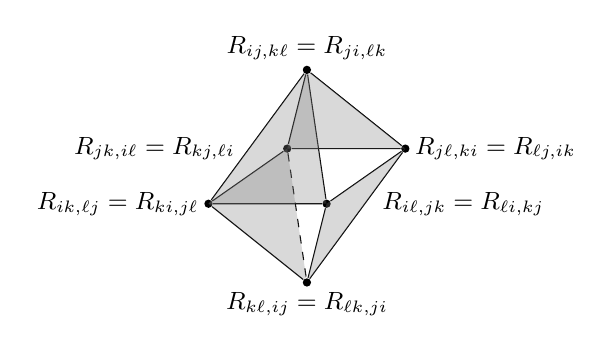
\begin{tikzpicture}
          \node [circ] (se) at (1.5, 0) {};
          \node [circ] (sw) at (0, 0) {};
          \node [circ] (ne) at (2.5, 0.7) {};
          \node [circ] (nw) at (1, 0.7) {};
          \node [circ] (top) at (1.25, 1.7) {};
          \node [circ] (bot) at (1.25, -1) {};

          \draw (sw) node [left] {\small $R_{ik, \ell j} = R_{ki, j\ell}$} -- (se) node [right] {\;\;\;\;\;\;\small $R_{i\ell, jk} = R_{\ell i, kj}$} -- (ne) node [right] {\small $R_{j\ell, ki} = R_{\ell j, ik}$} -- (nw) node [left] {\small $R_{jk, i\ell} = R_{kj, \ell i}$\;\;\;\;\;\;} -- (sw);

          \node [above] at (top) {\small $R_{ij, k\ell} = R_{ji, \ell k}$};
          \node [below] at (bot) {\small $R_{k\ell, ij} = R_{\ell k, ji}$};

          \draw (top) -- (sw) -- (bot);
          \draw (top) -- (se) -- (bot);
          \draw (top) -- (ne) -- (bot);

          \draw (top) -- (nw);
          \draw [dashed] (nw) -- (bot);

          \fill [opacity=0.3, gray] (top) -- (1.5, 0) -- (0, 0) -- (top);
          \fill [opacity=0.3, gray] (top) -- (2.5, 0.7) -- (1, 0.7) -- (top);

          \fill [opacity=0.3, gray] (bot) -- (1.5, 0) -- (2.5, 0.7) -- (bot);
          \fill [opacity=0.3, gray] (bot) -- (0, 0) -- (1, 0.7) -- (bot);
        \end{tikzpicture}
      \end{center}
      The equalities on each vertex is given by (i). By the first Bianchi identity, for each greyed triangle, the sum of the three vertices is zero.

      Now looking at the upper half of the octahedron, adding the two greyed triangles shows us the sum of the vertices in the horizontal square is $(-2) R_{ij, k\ell}$. Looking at the bottom half, we find that the sum of the vertices in the horizontal square is $(-2)R_{k\ell, ij}$. So we must have
      \[
        R_{ij, k\ell} = R_{k\ell, ij}.\qedhere
      \]
  \end{enumerate}
\end{proof}
What exactly are the properties of the Levi-Civita connection that make these equality works? The first equality of (i) did not require anything. The second equality of (i) required the compatibility with the metric, and (ii) required the symmetric property. The last one required both properties.

We can express the last property as saying $R_{ij, k\ell}$ is a symmetric bilinear form on $\Lambda^2 T_p^*M$. It is a straightforward exercise to rewrite the statement of this proposition in coordinate free notation using test vector fields. For example, the first equality in (i) can be written as
\[
  R(X, Y) = -R(Y, X).
\]
\subsubsection*{Sectional curvature}
The full curvature tensor is rather scary. So it is convenient to obtain some simpler quantities from it. Recall that if we had tangent vectors $X, Y$, then we can form
\[
  |X \wedge Y| = \sqrt{g(X, X)g(Y, Y) - g(X, Y)^2},
\]
which is the area of the parallelogram spanned by $X$ and $Y$. We now define
\[
  K(X, Y) = \frac{R(X, Y, X, Y)}{|X \wedge Y|^2}.
\]
Note that this is invariant under (non-zero) scaling of $X$ or $Y$, and is symmetric in $X$ and $Y$. Finally, it is also invariant under the transformation $(X, Y) \mapsto (X + \lambda Y, Y)$.

But it is an easy linear algebra fact that these transformations generate all isomorphism from a two-dimensional vector space to itself. So $K(X, Y)$ depends only on the $2$-plane spanned by $X, Y$. So we have in fact defined a function on the Grassmannian of $2$-planes, $K: \Gr(2, T_p M) \to \R$. This is called the \term{sectional curvature} (of $g$).

It turns out the sectional curvature determines the Riemann curvature tensor completely!
\begin{lemma}
  Let $V$ be a real vector space of dimension $\geq 2$. Suppose $R', R'': V^{\otimes 4} \to \R$ are both linear in each factor, and satisfies the symmetries we found for the Riemann curvature tensor. We define $K', K'': \Gr(2, V) \to \R$ as in the sectional curvature. If $K' = K''$, then $R' = R''$.
\end{lemma}
This is really just linear algebra.
\begin{proof}
  For any $X, Y, Z \in V$, we know
  \[
    R'(X + Z, Y, X + Z, Y) = R''(X + Z, Y, X + Z, Y).
  \]
  Using linearity of $R'$ and $R''$, and cancelling equal terms on both sides, we find
  \[
    R'(Z, Y, X, Y) + R'(X, Y, Z, Y) = R''(Z, Y, X, Y) + R''(X, Y, Z, Y).
  \]
  Now using the symmetry property of $R'$ and $R''$, this implies
  \[
    R'(X, Y, Z, Y) = R''(X, Y, Z, Y).
  \]
  Similarly, we replace $Y$ with $Y + T$, and then we get
  \[
    R'(X, Y, Z, T) + R'(X, T, Z, Y) = R''(X, Y, Z, Y) + R''"(X, T, Z, Y).
  \]
  We then rearrange and use the symmetries to get
  \[
    R'(X, Y, Z, T) - R''(X, Y, Z, T) = R'(Y, Z, X, T) - R''(Y, Z, X, T).
  \]
  We notice this equation says $R'(X, Y, Z, T) - R''(X, Y, Z, T)$ is invariant under the cyclic permutation $X \to Y \to Z \to X$. So by the first Bianchi identity, we have
  \[
    3(R'(X, Y, Z, T) - R''(X, Y, Z, T)) = 0.
  \]
  So we must have $R' = R''$.
\end{proof}

\begin{cor}
  Let $(M, g)$ be a manifold such that for all $p$, the function $K_p: \Gr(2, T_p M) \to \R$ is a constant map. Let
  \[
    R^0_p (X, Y, Z, T) = g_p(X, Z) g_p(Y, T) - g_p(X, T) g_p(Y, Z).
  \]
  Then
  \[
    R_p= K_p R_p^0.
  \]
  Here $K_p$ is just a real number, since it is constant. Moreover, $K_p$ is a smooth function of $p$.
\end{cor}

\begin{proof}
  We apply the previous lemma as follows: we define $R' = K_p R_p^0$ and $R'' = R_p$. It is a straightforward inspection to see that this $R^0$ does follow the symmetry properties of $R_p$, and that they define the same sectional curvature. So $R'' = R'$. We know $K_p$ is smooth in $p$ as both $g$ and $R$ are smooth.
\end{proof}
We can further show that if $\dim M > 2$, then $K_p$ is in fact independent of $p$ under the hypothesis of this function, and the proof requires a second Bianchi identity. This can be found on the first example sheet.

When does the condition of the corollary hold? We pick an \emph{orthonormal} basis, and express $R$ in coordinates $R_{ij, k\ell}$. Then writing $k = K_p$, the hypothesis holds iff
\[
  R_{ij, k\ell} = k(\delta_{ik}\delta_{j\ell} - \delta_{i\ell} \delta_{jk})
\]
iff
\[
  R_{ij, ij} = - R_{ij, ji} = k,
\]
and all other entries all zero.

\subsubsection*{Other curvatures}
There are other quantities we can extract out of the curvature, which will later be useful.
\begin{defi}[Ricci curvature]\index{Ricci curvature}\index{curvature!Ricci}
  The \emph{Ricci curvature} of $g$ at $p \in M$ is
  \[
    \Ric_p(X, Y) = \tr(v \mapsto R_p(X, v) Y).
  \]
  In terms of coordinates, we have
  \[
    \Ric_{ij} = R^q_{i,jq} = g^{pq} R_{pi, jq},
  \]
  where $g^{pq}$ denotes the inverse of $g$, and we implicitly sum over repeated indices.

  This $\Ric$ is a symmetric bilinear form on $T_p M$. This can be determined by the quadratic form
  \[
    \Ric(X) = \frac{1}{n - 1} \Ric_p(X, X).
  \]
  The coefficient $\frac{1}{n - 1}$ is just a convention.
\end{defi}
There are still two indices we can contract, and we can define
\begin{defi}[Scalar curvature]\index{scalar curvature}\index{scalar curvature}
  The \emph{scalar curvature} of $g$ is the trace of $\Ric$ respect to $g$. Explicitly, this is defined by
  \[
    s = g^{ij}\Ric_{ij} = g^{ij} R^q_{i, jq} = R^{qi}\!_{iq}.
  \]
\end{defi}
Sometimes a convention is to define the scalar curvature as $\frac{s}{n(n - 1)}$ instead.

In the case of a constant sectional curvature tensor, we have
\[
  \Ric_p = (n - 1) K_p g_p,
\]
and
\[
  s(p) = n(n - 1) K_p.
\]

\subsubsection*{Low dimensions}
If $n = 2$, ie. we have surfaces, then the Riemannian metric $g$ is also known as the \term{first fundamental form}, and it is usually written as
\[
  g = E\;\d u^2 + 2 F \;\d u\;\d v + G \;\d v^2.
\]
Up to the symmetries, the only non-zero component of the curvature tensor is $R_{12, 12}$, and using the definition of the scalar curvature, we find
\[
  R_{12,12} = \frac{1}{2} s (EG - F^2).
\]
Thus $s/2$ is also the sectional curvature (there can only be one plane in the tangent space, so the sectional curvature is just a number). One can further check that
\[
  \frac{s}{2} = K = \frac{LN - M^2}{EG - F^2},
\]
the \term{Gaussian curvature}. We see that in two dimensions, there is only one independent component of the Gaussian curvature. Also, $R_{12, 21}$ is the determinant of the second fundamental form.

If $n = 3$, one can check that $R(g)$ is determined by the Ricci curvature.

\section{Geodesics}
\subsection{Definitions and basic properties}
We will eventually want to talk about geodesics. However, the set up we need to write down the definition of geodesics can be done in a much more general way, and we will do that.

The general setting is that we have a vector bundle $\pi: E \to M$. 
\begin{defi}[Lift]\index{lift}
  Let $\pi: E \to M$ be a vector bundle with typical fiber $V$. Consider a curve $\gamma: (-\varepsilon, \varepsilon) \to M$. A \emph{lift} of $\gamma$ is a map $\gamma^E: (-\varepsilon, \varepsilon) \to E$ if $\pi \circ \gamma^E = \gamma$, ie. the following diagram commutes:
  \[
    \begin{tikzcd}
      & E \ar[d, "\pi"]\\
      (-\varepsilon, \varepsilon) \ar[r, "\gamma"] \ar[ur, "\gamma^E"] & M
    \end{tikzcd}.
  \]
\end{defi}
For $p \in M$, we write $E_p = \pi^{-1}(\{p\}) \cong V$ for the fiber above $p$. We can think of $E_p$ as the space of some ``information'' at $p$. For example, if $E = TM$, then the ``information'' is a tangent vector at $p$. In physics, the manifold $M$ might represent our universe, and a point in $E_p$ might be the value of the electromagnetic field at $p$.

Thus, given a path $\gamma$ in $M$, a lift corresponds to providing that piece of ``information'' at each point along the curve. For example, if $E = TM$, then we can canonically produce a lift of $\gamma$, given by taking the derivative of $\gamma$ at each point.

Locally, suppose we are in some coordinate neighbourhood $U \subseteq M$ such that $E$ is trivial on $U$. After picking a trivialization, we can write our lift as
 Then $\gamma^E$ is of the form
\[
  \gamma^E(t) = (\gamma(t), a(t))
\]
for some function $a: (-\varepsilon, \varepsilon) \to V$.

One thing we would want to do with such lifts is to differentiate them, and see how it changes along the curve. When we have a \emph{section} of $E$ on the whole of $M$ (or even just an open neighbourhood), rather than just a lift along a curve, the connection provides exactly the information needed to do so. It is not immediately obvious that the connection also allows us to differentiate curves along paths, but it does.

\begin{prop}
  Let $\gamma: (-\varepsilon, \varepsilon) \to M$ be a curve. Then there is a uniquely determined operation $\frac{\nabla}{\d t}$ from the space of all lifts of $\gamma$ to itself, satisfying the following conditions:
  \begin{enumerate}
    \item For any $c, d \in \R$ and lifts $\tilde{\gamma}^E, \gamma^E$ of $\gamma$, we have.
      \[
        \frac{\nabla}{\d t}(c\gamma^E + d \tilde{\gamma}^E) = c\frac{\nabla \gamma^E}{\d t} + d \frac{\nabla \tilde{\gamma}^E}{\d t}
      \]
    \item For any lift $\gamma^E$ of $\gamma$ and function $f: (-\varepsilon, \varepsilon) \to \R$, we have
      \[
        \frac{\nabla}{\d t}(f \gamma^E) = \frac{\d f}{\d t} + f \frac{\nabla \gamma^E}{\d t}.
      \]
    \item If there is a local section $s$ of $E$ and a local vector field $V$ on $M$ such that
      \[
        \gamma^E(t) = s(\gamma(t)),\quad \dot{\gamma}(t) = V(\gamma(t)),
      \]
      then we have
      \[
        \frac{\nabla \gamma^E}{\d t} = (\nabla_V s) \circ \gamma.
      \]
  \end{enumerate}
  Locally, this is given by
  \[
    \left(\frac{\nabla \gamma^E}{\d t}\right)^i = \dot{a}^i + \Gamma^i_{jk} a^j \dot{x}^k.
  \]
\end{prop}
The proof is straightforward --- one just checks that the local formula works, and the three properties force the operation to be locally given by that formula.

\begin{defi}[Covariant derivative]\index{covariant derivative}
  The uniquely defined operation in the proposition above is called the \emph{covariant derivative}.
\end{defi}

In some sense, lifts that have vanishing covariant derivative are ``constant'' along the map.

\begin{defi}[Horizontal lift]\index{horizontal lift}\index{lift!horizontal}
  Let $\nabla$ be a connection on $E$ with $\Gamma^i_{jk}(x)$ the coefficients in a local trivialization. We say a lift $\gamma^E$ is \emph{horizontal} if
  \[
    \frac{\nabla \gamma^E}{\d t} = 0.
  \]
\end{defi}
Since this is a linear first-order ODE, we know that for a fixed $\gamma$, given any initial $a(0) \in E_{\gamma(0)}$, there is a unique way to obtain a horizontal lift.

\begin{defi}[Parallel transport]\index{parallel transport}
  Let $\gamma : [0, 1] \to M$ be a curve in $M$. Given any $a_0 \in E_{\gamma(0)}$, the unique horizontal lift of $\gamma$ with $\gamma^E(0) = (\gamma(0), a_0)$ is called the \emph{parallel transport} of $a_0$ along $\gamma(0)$. We sometimes also call $\gamma^E(1)$ the parallel transport.
\end{defi}
Of course, we want to use this general theory to talk about the case where $M$ is a Riemannian manifold, $E = TM$ and $\nabla$ is the Levi-Civita connection of $g$. In this case, each curve $\gamma(t)$ has a canonical lift independent of the metric or connection given simply by taking the derivative $\dot{\gamma}(t)$.
\begin{defi}[Geodesic]\index{geodesic}
  A curve $\gamma(t)$ on a Riemannian manifold $(M, g)$ is called a \emph{geodesic curve} if its canonical lift is horizontal with respect to the Levi-Civita connection. In other words, we need
  \[
    \frac{\nabla \dot{\gamma}}{\d t} = 0.
  \]
\end{defi}
In local coordinates, we write this condition as
\[
  \ddot{x}_i + \Gamma^i_{jk}\dot{x}^j \dot{x}^k = 0.
\]
This time, we obtain a second-order ODE. So a geodesic is uniquely specified by the initial conditions $p = x(0)$ and $a = \dot{x}(0)$. We will denote the resulting geodesic as $\gamma_p(t; a)$, where $t$ is the time coordinate as usual.

Since we have a non-linear ODE, existence is no longer guaranteed on all time, but just for some interval $(-\varepsilon, \varepsilon)$. Of course, we still have uniqueness of solutions.

We now want to prove things about geodesics. To do so, we will need to apply some properties of the covariant derivative we just defined. Since we are lazy, we would like to reuse results we already know about the covariant derivative for vector fields. The trick is to notice that locally, we can always extend $\dot{\gamma}$ to a vector field.

Indeed, we work in some coordinate chart around $\gamma(0)$, and we wlog assume
\[
  \dot{\gamma}(0) = \frac{\partial}{\partial x_1}.
\]
By the inverse function theorem, we note that $x_1(t)$ is invertible near $0$, and we can write $t = t(x_1)$ for small $x_1$. Then in this neighbourhood of $0$, we can view $x_k$ as a function of $x_1$ instead of $t$. Then we can define the vector field
\[
  \dot{\underline{\gamma}}(x_1, \cdots, x_k) = \dot{\gamma}(x_1, x_2(x_1), \cdots, x_k(x_1)).
\]
By construction, this agrees with $\dot{\gamma}$ along the curve.

Using this notation, the geodesic equation can be written as
\[
  \left.\nabla_{\dot{\underline{\gamma}}} \dot{\underline{\gamma}}\right|_{\gamma(t)} = 0,
\]
where the $\nabla$ now refers to the covariant derivative of vector fields, ie. the connection itself.
\begin{center}
  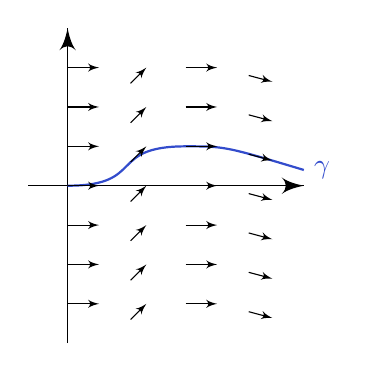
\begin{tikzpicture}
    \draw [->] (-0.5, 0) -- (3, 0);
    \draw [->] (0, -2) -- (0, 2);

    \draw [mblue, thick] (0, 0) .. controls (1, 0) and (0.5, 0.5) .. (1.5, 0.5) .. controls (2, 0.5) .. (3, 0.2) node [right] {$\gamma$};

    \foreach \x in {-1.5, -1, -0.5, 0, 0.5, 1, 1.5} {
      \begin{scope}[shift={(0, \x)}]
        \draw [-latex'] (0, 0) -- +(0.4, 0) ;
        \draw [-latex'] (0.8, -0.2) -- +(0.2, 0.2) ;
        \draw [-latex'] (1.5, 0) -- +(0.4, 0) ;
        \draw [-latex'] (2.3, -0.1) -- +(0.3, -0.08) ;
      \end{scope}
    }
  \end{tikzpicture}
\end{center} % improve picture
Using this, a lot of the desired properties of geodesics immediately follow from well-known properties of the covariant derivative. For example,
\begin{prop}
  If $\gamma$ is a geodesic, then $|\dot{\gamma}(t)|_g$ is constant.
\end{prop}

\begin{proof}
  We use the extension $\dot{\underline{\gamma}}$ around $p = \gamma(0)$, and stop writing the underlines. Then we have
  \[
    \dot{\gamma}(g(\dot{\gamma}, \dot{\gamma})) = g(\nabla_{\dot{\gamma}} \dot{\gamma}, \dot{\gamma})+ g(\dot{\gamma}, \nabla_{\dot{\gamma}} \dot{\gamma}) = 0,
  \]
  which is valid at each $q = \gamma(t)$ on the curve. But at each $q$, we have
  \[
    \dot{\gamma}(g(\dot{\gamma}, \dot{\gamma})) = \dot{x}^k \frac{\partial}{\partial x_k} g(\dot{\gamma}, \dot{\gamma}) = \frac{\d}{\d t} |\dot{\gamma}(t)|_g^2
  \]
  by the chain rule. So we are done.
\end{proof}

At this point, it might be healthy to look at some examples of geodesics.
\begin{eg}
  In $\R^n$ with the Euclidean metric, we have $\Gamma^i_{jk} = 0$. So the geodesic equation is
  \[
    \ddot{x}_k = 0.
  \]
  So the geodesics are just straight lines.
\end{eg}

\begin{eg}
  On a sphere $S^n$ with the usual metric induced by the standard embedding $S^n \hookrightarrow \R^{n + 1}$. Then the geodesics are great circles.

  To see this, we may wlog $p = e_0$ and $a = e_1$, for a standard basis $\{e_i\}$ of $\R^{n + 1}$. We can look at the map
  \[
    \varphi: (x_0, \cdots, x_n) \mapsto (x_0, x_1, -x_2, \cdots, -x_n),
  \]
  and it is clearly an isometry of the sphere. Therefore it preserves the Riemannian metric, and hence sends geodesics to geodesics. Since it also preserves $p$ and $a$, we know $\varphi(\gamma) = \gamma$ by uniqueness. So it must be contained in the great circle lying on the plane spanned by $e_0$ and $e_1$.
\end{eg}

\begin{lemma}
  Let $p \in M$, and $a \in T_p M$. As before, let $\gamma_p(t, a)$ be the geodesic with $\gamma(0) = p$ and $\dot{\gamma}(0) = p$. Then
  \[
    \gamma_p(\lambda t, a) = \gamma_p(t, \lambda a),
  \]
  and in particular is a geodesic.
\end{lemma}

\begin{proof}
  We apply the chain rule to get
  \begin{align*}
    \frac{\d}{\d t} \gamma(\lambda t, a) &= \lambda \dot{\gamma} (\lambda t, a)\\
    \frac{\d^2}{\d t^2} \gamma(\lambda t, a) &= \lambda^2 \ddot{\gamma}(\lambda t, a).
  \end{align*}
  So $\gamma(\lambda t, a)$ satisfies the geodesic equations, and have initial velocity $\lambda a$. Then we are done by uniqueness of ODE solutions.
\end{proof}

Thus, instead of considering $\gamma_p(t, a)$ for arbitrary $t$ and $a$, we can just fix $t = 1$, and look at the different values of $\gamma_p(1, a)$. By ODE theorems, we know this depends smoothly on $a$, and is defined on some open neighbourhood of $0 \in T_p M$.

\begin{defi}[Exponential map]\index{exponential map}
  Let $(M, g)$ be a Riemannian manifold, and $p \in M$. We define $\exp_p$ by
  \[
    \exp_p(a) = \gamma(1, a) \in M
  \]
  for $a \in T_p M$ whenever this is defined.
\end{defi}

We know this function has domain at least some open ball around $0 \in T_p M$, and is smooth. Also, by construction, we have $\exp_p(0) = p$.

In fact, the exponential map gives us a chart around $p$ locally, known as \emph{geodesic local coordinates}. To do so, it suffices to note the following rather trivial proposition.

\begin{prop}
  We have
  \[
    (\d \exp_p)_0 = \id _{T_p M},
  \]
  where we identify $T_0 (T_p M) \cong T_p M$ in the natural way.
\end{prop}
All this is saying is if you go in the direction of $a \in T_p M$, then you go in the direction of $a$.

\begin{proof}
   \[
     (\d \exp_p)_0(v) = \frac{\d}{\d t} \exp_p(tv) = \frac{\d}{\d t} \gamma(1, tv) = \frac{\d}{\d t} \gamma(t, v) = v.
   \]
\end{proof}

\begin{cor}
  $\exp_p$ maps an open ball $B(0, \delta) \subseteq T_p M$ to $U \subseteq M$ diffeomorphically for some $\delta > 0$.
\end{cor}

\begin{proof}
  By the inverse mapping theorem.
\end{proof}

This tells us the inverse of the exponential map gives us a chart of $M$ around $p$. These coordinates are often known as \term{geodesic local coordinates}.

In these coordinates, the geodesics from $p$ have the very simple form
\[
  \gamma(t, a) = ta
\]
for all $a \in T_p M$ and $t$ sufficiently small that this makes sense.

Now consider a linear isometry $(T_p N, g(p)) \cong (\R^n, \mathrm{eucl})$, and under this identification, we have a map
\[
  (r, \mathbf{v}) \in (0, \delta) \times S^{n - 1} \mapsto \exp_p (r\mathbf{v}) \in M^n.
\]
This chart is known as \term{geodesic polar coordinates}. For each fixed $r$, the image of this map is called a \term{geodesic sphere} of geodesic radius $r$, written $\Sigma_r$\index{$\Sigma_r$}. This is an embedded submanifold of $M$.

Note that in geodesic local coordinates, the metric at $0 \in T_p N$ is given by the Euclidean metric. However, the metric at other points can be complicated. Fortunately, Gauss' lemma says it is not \emph{too} complicated.

\begin{thm}[Gauss' lemma]
  The geodesic spheres are perpendicular to their radii. More precisely, $\gamma_p(t, a)$ meets every $\Sigma_r$ orthogonally, whenever this makes sense. Thus we can write the metric in geodesic polars as
  \[
    g = \d r^2 + h(r, \mathbf{v}),
  \]
  where for each $r$, we have
  \[
    h(r, \mathbf{v}) = g|_{\Sigma_r}.
  \]
  In matrix form, we have
  \[
    g =
    \begin{pmatrix}
      1 & 0 & \cdots & 0\\
      0\\
      \rvdots & & h\\
      0
    \end{pmatrix}
  \]
\end{thm}

The proof is not hard, but it involves a few subtle points.
\begin{proof}
  We work in geodesic coordinates. It is clear that $g(\partial_r, \partial_r) = 1$.

  Consider an arbitrary vector field $X = X(\mathbf{v})$ on $S^{n - 1}$. This induces a vector field on some neighbourhood $B(0, \delta) \subseteq T_p M$ by
  \[
    \tilde{X}(r\mathbf{v}) = X(\mathbf{v}).
  \]
  Pick a direction $\mathbf{v} \in T_pM$, and consider the unit speed geodesic $\gamma$ in the direction of $\mathbf{v}$. We define
  \[
    G(r) = g(\tilde{X}(r\mathbf{v}), \dot{\gamma}(r)) = g(\tilde{X}, \dot{\gamma}(r)).
  \]
  We begin by noticing that
  \[
    \nabla_{\partial_r} \tilde{X} - \nabla_{\tilde{X}} \partial_r = [\partial_r , \tilde{X}] = 0.
  \]
  So we have
  \[
    \frac{\d}{\d r} G(r) = g(\nabla_{\dot{\gamma}} \tilde{X}, \dot{\gamma}) + g(\tilde{X}, \nabla_{\dot{\gamma}} \dot{\gamma}).
  \]
  We know the second term vanishes, since $\gamma$ is a geodesic. Noting that $\dot{\gamma} = \frac{\partial}{\partial r}$, we know the first term is equal to
  \[
    g(\nabla_{\tilde{X}} \partial_r, \partial_r) = \frac{1}{2} \Big(g(\nabla_{\tilde{X}} \partial_r, \partial_r) + g( \partial_r, \nabla_{\tilde{X}}\partial_r)\Big) = \frac{1}{2} \tilde{X} (g(\partial_r, \partial_r)) = 0,
  \]
  since we know that $g(\partial_r, \partial_r) = 1$ constantly.

  Thus, we know $G(r)$ is constant. But $G(0) = 0$ since the metric at $0$ is the Euclidean metric. So $G$ vanishes everywhere, and so $\partial_r$ is perpendicular to $\Sigma_g$.

%
% We work in the geodesic coordinates. Consider an arbitrary vector field $X = X(\mathbf{v}) \in \Vect(S^{n - 1})$. Identifying $S^{n - 1} \subseteq T_p M$, we extend this to a vector field on $B(0,\delta) \subseteq T_p M$ by
% \[
% \tilde{X}(r\mathbf{v}) = r X(\mathbf{v}).
% \]
% We want to show that $\tilde{X}$ is perpendicular $\frac{\partial}{\partial r}$ at each point in $B \setminus \{0\}$. Consider an arbitrary unit speed geodesic $\gamma$ in direction $\mathbf{v}$. We define the quantity
% \[
% G(r) = g(\tilde{X}(r\mathbf{v}), \dot{\gamma}(r)).
% \]
% We will show that $G$ vanishes everywhere. To do so, we claim that
% \[
% \frac{\d G}{\d r} = \frac{G}{r}.
% \]
% It then follows that $G$ is linear in $r$,
%
%
% This is equivalent to showing that it is perpendicular to $\dot{\gamma}$. Recall that we have
% \[
% \nabla_{\dot{\gamma}} \dot{\gamma} = 0
% \]
% by definition. Also, we know $\frac{\partial}{\partial r}$ has unit norm. Thus to show that
% \[
% g(\tilde{X}, \dot{\gamma}) = 0
% \]
%
% We consider
% \[
% \nabla_{\partial/\partial r} \tilde{X} - \nabla_{\tilde{X}} \frac{\partial}{\partial r} = \left[\frac{\partial}{\partial r}, \tilde{X}\right] = \frac{\d}{\d r}\tilde{X} = \frac{\tilde{X}}{r}.
% \]
% We also have
% \begin{align*}
% \frac{\d}{\d r} (g(\tilde{X}, \dot{\gamma})) &= g(\nabla_{\dot{\gamma}} \tilde{X}, \dot{\gamma}) + g(\tilde{X}, \nabla_{\dot{\gamma}} \dot{\gamma})\\
% &= -g\left(\nabla_{\tilde{X}} \dot{\gamma} + \frac{\tilde{X}}{r}, \dot{\gamma}\right) = \frac{1}{r} g(Y, \dot{~g}),
% \end{align*}
% noting that $g(\nabla_{\tilde{X}} \dot{\gamma}, \dot{\gamma}) = Y g(\dot{\gamma}, \dot{\gamma}) = 0$ since $|\dot{\gamma}|$ is constant along spheres. We define
% \[
% G = g(\tilde{X}, \dot{\gamma}).
% \]
% Then we know this satisfies
% \[
% \frac{\d}{\d r} G = \frac{G}{r}.
% \]
% This is a very simple ODE in $r$, and this tells us $G$ is linear in $r$. So
% \[
% \frac{\d G}{\d r}
% \]
% is independent of $r$. But as $r \to 0$, we know
% \[
% \lim_{r \to 0} \frac{\d G}{\d r} = \lim_{r \to 0} g\left(X, \frac{\partial}{\partial r}\right) = 0.
% \]
\end{proof}

\begin{cor}
  Let $a, w \in T_p M$. Then
  \[
    g((\d \exp_p)_a a, (\d \exp_p)_a w) = g(a, w)
  \]
  whenever $a$ lives in the domain of the geodesic local neighbourhood.
\end{cor}

\subsection{Jacobi fields}
Fix a Riemannian manifold $M$. Let's imagine that we have a ``manifold'' of all smooth curves on $M$. Then this ``manifold'' has a ``tangent space''. Morally, given a curve $\gamma$, a ``tangent vector'' at $\gamma$ in the space of curve should correspond to providing a tangent vector (in $M$) at each point along $\gamma$:
\begin{center}
  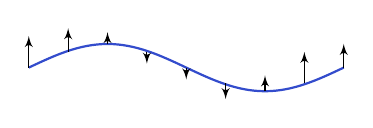
\begin{tikzpicture}
    \draw [mblue, thick] (0, 0) sin (1, 0.3) cos (2, 0) sin (3, -0.3) cos (4, 0);

    \draw [-latex'] (0, 0) -- +(0, 0.4);
    \draw [-latex'] (0.5, 0.2) -- +(0, 0.3);
    \draw [-latex'] (1, 0.3) -- +(0, 0.15);
    \draw [-latex'] (1.5, 0.2) -- +(0, -0.15);
    \draw [-latex'] (2, 0) -- +(0, -0.15);
    \draw [-latex'] (2.5, -0.2) -- +(0, -0.2);
    \draw [-latex'] (3, -0.3) -- +(0, 0.2);
    \draw [-latex'] (3.5, -0.2) -- +(0, 0.4);
    \draw [-latex'] (4, 0) -- +(0, 0.3);
  \end{tikzpicture}
\end{center}
Since we are interested in the geodesics only, we consider the ``submanifold'' of geodesics curves. What are the corresponding ``tangent vectors'' living in this ``submanifold''?

In rather more concrete terms, suppose $f_s(t) = f(t, s)$ is a family of geodesics in $M$ indexed by $s \in (-\varepsilon, \varepsilon)$. What do we know about $\left.\frac{\partial f}{\partial s}\right|_{s = 0}$, a vector field along $f_0$?

We begin by considering such families that fix the starting point $f(0, s)$, and then derive some properties of $\frac{\partial f}{\partial s}$ in these special cases. We will then define a \emph{Jacobi field} to be any vector field along a curve that satisfies these properties. We will then prove that these are exactly the variations of geodesics.

Suppose $f(t, s)$ is a family of geodesics such that $f(0, s) = p$ for all $s$. Then in geodesics local coordinates, it must look like this:
\begin{center}
  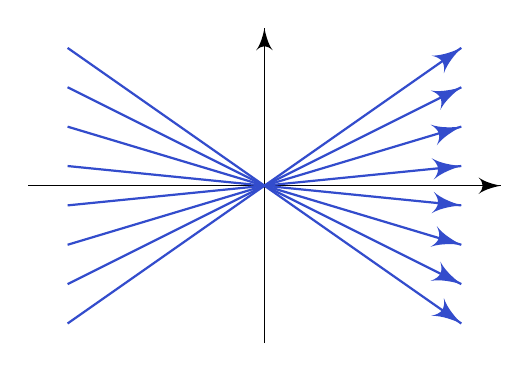
\begin{tikzpicture}
    \draw [->] (-3, 0) -- (3, 0);
    \draw [->] (0, -2) -- (0, 2);
    \foreach \y in {-1.75,-1.25,-0.75,-0.25,0.25,0.75,1.25,1.75} {
      \draw [->, mblue, thick] (-2.5, -\y) -- (2.5, \y);
    }
  \end{tikzpicture}
\end{center}
For a fixed $p$, such a family is uniquely determined by a function
\[
  a(s): (-\varepsilon, \varepsilon) \to T_p M
\]
such that
\[
  f(t, s) = \exp_p(t a(s)).
\]
The initial conditions of this variation can be given by $a(0) = a$ and 
\[
  \dot{a}(0) = w \in T_a(T_p M) \cong T_p M.
\]
We would like to know the ``variation field'' of $\gamma(t) = f(t, 0) = \gamma_p(t, a)$ this induces. In other words, we want to find $\frac{\partial f}{\partial s} (t, 0)$. This is not hard. It is just given by
\[
  (\d \exp_p)_{t a_0} (tw) = \frac{\partial f}{\partial s}(t, 0),
\]
As before, to prove something about $f$, we want to make good use of the properties of $\nabla$. Locally, we extend the vectors $\frac{\partial f}{\partial s}$ and $\frac{\partial f}{\partial t}$ to vector fields $\frac{\partial}{\partial t}$ and $\frac{\partial}{\partial s}$. Then in this set up, we have
\[
  \dot{\gamma} = \frac{\partial f}{\partial t} = \frac{\partial}{\partial t}.
\]
Note that in $\frac{\partial f}{\partial t}$, we are differentiating $f$ with respect to $t$, whereas the $\frac{\partial}{\partial t}$ on the far right is just a formal expressions.

By the geodesic equation, we have
\[
  0 = \frac{\nabla}{\d t} \dot{\gamma} = \Delta_{\partial_t} \partial_t.
\]
Therefore, using the definition of the curvature tensor $R$, we obtain
\begin{align*}
  0 = \nabla_{\partial_s} \nabla_{\partial_t} \frac{\partial}{\partial t} &= \nabla_{\partial_t} \nabla_{\partial_s} \partial_t - R(\partial_s, \partial_t) \partial_t\\
  &= \nabla_{\partial_t} \nabla_{\partial_s} \partial_t + R(\partial_t, \partial_s) \partial_t
\end{align*}
We let this act on the function $f$. So we get
\[
  0 = \frac{\nabla}{\d t} \frac{\nabla}{\d s} \frac{\partial f}{\partial t} + R(\partial_t, \partial_s) \frac{\partial f}{\partial t}.
\]
We write
\[
  J(t) = \frac{\partial f}{\partial s}(t, 0),
\]
which is a vector field along the geodesic $\gamma$. Using the fact that
\[
  \frac{\nabla}{\d s} \frac{\partial f}{\partial t} = \frac{\nabla}{\d t} \frac{\partial f}{\partial s},
\]
we find that $J$ must satisfy the ordinary differential equation
\[
  \frac{\nabla^2}{\d t^2} J + R(\dot{\gamma}, J) \dot{\gamma} = 0.
\]
This is a linear second-order ordinary differential equation.

\begin{defi}[Jacobi field]\index{Jacobi field}
  Let $\gamma: [0, L] \to M$ be a geodesic. A \emph{Jacobi field} is a vector field $J$ along $\gamma$ that is a solution of the \term{Jacobi equation} on $[0, L]$
  \[
    \frac{\nabla^2}{\d t^2} J + R(\dot{\gamma}, J) \dot{\gamma} = 0. \tag{$\dagger$}
  \]
\end{defi}

We now embark on a rather technical journey to prove results about Jacobi fields. Observe that $\dot{\gamma}(t)$ and $t \dot{\gamma}(t)$ both satisfy this equation, rather trivially.
\begin{thm}
  Let $\gamma: [0, L] \to N$ be a geodesic in a Riemannian manifold $(M, g)$. Then
  \begin{enumerate}
    \item For any $u, v \in T_{\gamma(0)}M$, there is a unique Jacobi field $J$ along $\Gamma$ with
      \[
        J(0) = u,\quad \frac{\nabla J}{\d t}(0) = v.
      \]
      If
      \[
        J(0) = 0,\quad \frac{\nabla J}{\d t}(0) = k \dot{\gamma}(0),
      \]
      then $J(t) = kt \dot{\gamma}(t)$. Moreover, if both $J(0), \frac{\nabla J}{\d t}(0)$ are orthogonal to $\dot{\gamma}(0)$, then $J(t)$ is perpendicular to $\dot{\gamma}(t)$ for all $[0, L]$.

      In particular, the vector space of all Jacobi fields along $\gamma$ have dimension $2n$, where $n = \dim M$.

      The subspace of those Jacobi fields pointwise perpendicular to $\dot{\gamma}(t)$ has dimensional $2(n - 1)$.
    \item $J(t)$ is independent of the parametrization of $\dot{\gamma}(t)$. Explicitly, if $\tilde{\gamma}(t) = \tilde{\gamma}(\lambda t)$, then $\tilde{J}$ with the same initial conditions as $J$ is given by
      \[
        \tilde{J}(\tilde{\gamma}(t)) = J(\gamma(\lambda t)).
      \]
  \end{enumerate}
\end{thm}

This is the kind of theorem whose statement is longer than the proof.
\begin{proof}\leavevmode
  \begin{enumerate}
    \item Pick an orthonormal basis $e_1,\cdots, e_n$ of $T_p M$, where $p = \gamma(0)$. Then parallel transports $\{X_i(t)\}$ via the Levi-Civita connection preserves the inner product.

      We take $e_1$ to be parallel to $\dot{\gamma}(0)$. By definition, we have
      \[
        X_i(0) = e_i,\quad \frac{\nabla X_i}{\d t} = 0.
      \]
      Now we can write
      \[
        J = \sum_{i = 1}^n y_i X_i.
      \]
      Then taking $g(X_i, \ph)$ of $(\dagger)$ , we find that
      \[
        \ddot{y}_i + \sum_{j = 2}^n R(\dot{\gamma}, X_j, \dot{\gamma}, X_i) y_j = 0.
      \]
      Then the claims of the theorem follow from the standard existence and uniqueness of solutions of differential equations.

      In particular, for the orthogonality part, we know that $J(0)$ and $\frac{\nabla J}{\d t}(0)$ being perpendicular to $\dot{\gamma}$ is equivalent to $y_1(0) = \dot{y}_1 (0) = 0$, and then Jacobi's equation gives
      \[
        \ddot{y}_1(t) = 0.
      \]
    \item This follows from uniqueness.\qedhere
  \end{enumerate}
\end{proof}

Our discussion of Jacobi fields so far has been rather theoretical. Now that we have an explicit equation for the Jacobi field, we can actually produce some of them. We will look at the case where we have constant sectional curvature.

\begin{eg}
  Suppose the sectional curvature is constantly $K \in \R$, for $\dim M \geq 3$. We wlog $|\dot{\gamma}| = 1$. We let $J$ along $\gamma$ be a Jacobi field, normal to $\dot{\gamma}$.

  Then for any vector field $T$ along $\gamma$, we have
  \[
    \bra R(\dot{\gamma}, J) \dot{\gamma}, T\ket = K(g(\dot{\gamma}, \dot{\gamma}) g(J, T) - g(\dot{\gamma}, J) g(\dot{\gamma}, T)) = K g(J, T).
  \]
  Since this is true for all $T$, we know
  \[
    R(\dot{\gamma}, J) \dot{\gamma} = KJ.
  \]
  Then the Jacobi equation becomes
  \[
    \frac{\nabla^2}{\d t^2}J + KJ = 0.
  \]
  So we can immediately write down a collection of solutions
  \[
    J(t) =
    \begin{cases}
      \frac{\sin(t \sqrt{K})}{\sqrt{K}} X_i(t) & K > 0\\
      t X_i(t) & K = 0\\
      \frac{\sinh(t \sqrt{-K})}{\sqrt{-K}} X_i(t) & K < 0
    \end{cases}.
  \]
  for $i = 2, \cdots, n$, and this has initial conditions
  \[
    J(0) = 0,\quad \frac{\nabla J}{\d t}(0) = e_i.
  \]
  Note that these Jacobi fields vanishes at $0$.
\end{eg}

We can now deliver our promise, proving that Jacobi fields are precisely the variations of geodesics.
\begin{prop}
  Let $\gamma: [a, b] \to M$ be a geodesic, and $f(t, s)$ a variation of $\gamma(t) = f(t, 0)$ such that $f(t, s) = \gamma_s(t)$ is a geodesic for all $|s|$ small. Then
  \[
    J(t) = \frac{\partial f}{\partial s}
  \]
  is a Jacobi field along $\dot{\gamma}$.

  Conversely, every Jacobi field along $\gamma$ can be obtained this way for an appropriate function $f$.
\end{prop}

\begin{proof}
  The first part is just the exact computation as we had at the beginning of the section, but for the benefit of the reader, we will reproduce the proof again.
  \begin{align*}
    \frac{\nabla^2 J}{\d t} &= \nabla_t \nabla_t \frac{\partial f}{\partial s}\\
    &= \nabla_t \nabla_s \frac{\partial f}{\partial t}\\
    &= \nabla_s \left(\nabla_t \frac{\partial f}{\partial t}\right) - R(\partial_t, \partial_s) \dot{\gamma}_s.
  \end{align*}
  We notice that the first term vanishes, because $\nabla_t \frac{\partial f}{\partial t} = 0$ by definition of geodesic. So we find
  \[
    \frac{\nabla^2 J}{\d t} = -R(\dot{\gamma}, J) \dot{\gamma},
  \]
  which is the Jacobi equation.

  The converse requires a bit more work. We will write $J'(0)$ for the covariant derivative of $J$ along $\gamma$. Given a Jacobi field $J$ along a geodesic $\gamma(t)$ for $t \in [0, L]$, we let $\tilde{\gamma}$ be another geodesic such that
  \[
    \tilde{\gamma}(0) = \gamma(0),\quad \dot{\tilde{\gamma}}(0) = J(0).
  \]
  We take parallel vector fields $X_0, X_1$ along $\tilde{\gamma}$ such that
  \[
    X_0(0) = \dot{\gamma}(0),\quad X_1(0) = J'(0).
  \]
  We put $X(s) = X_0(s) + s X_1(s)$. We put
  \[
    f(t, s) = \exp_{\tilde{\gamma}(s)} (t X(s)). % insert a picture?
  \]
  In local coordinates, for each fixed $s$, we find
  \[
    f(t, s) = \tilde{\gamma}(s) + t X(s) + O(t^2)
  \]
  as $t \to 0$. Then we define
  \[
    \gamma_s(t) = f(t, s)
  \]
  whenever this makes sense. This depends smoothly on $s$, and the previous arguments say we get a Jacobi field
  \[
    \hat{J}(t) = \frac{\partial f}{\partial s}(t, 0)
  \]
  We now want to check that $\hat{J} = J$. Then we are done. To do so, we have to check the initial conditions. We have
  \[
    \hat{J}(0) = \frac{\partial f}{\partial s}(0, 0) = \frac{\d \tilde{\gamma}}{\d s}(0) = J(0),
  \]
  and also
  \[
    \hat{J}'(0) = \frac{\nabla}{\d t} \frac{\partial f}{\partial s}(0, 0) = \frac{\nabla}{\d s} \frac{\partial f}{\partial t}(0, 0) = \frac{\nabla X}{\d s}(0) = X_1(0) = J'(0).
  \]
  So we have $\hat{J} = J$.
\end{proof}

\begin{cor}
  Every Jacobi field $J$ along a geodesic $\gamma$ with $J(0) = 0$ is given by
  \[
    J(t) = (\d \exp_p)_{t \dot{\gamma}(0)} (t J'(0))
  \]
  for all $t \in [0, L]$.
\end{cor}
This is just a reiteration of the fact that if we pull back to the geodesic local coordinates, then the variation must look like this:
\begin{center}
  \begin{tikzpicture}
    \draw [->] (-3, 0) -- (3, 0);
    \draw [->] (0, -2) -- (0, 2);
    \draw [mblue, thick] (-2.5, 0) -- (2.5, 0);
    \draw [mblue, thick] (-2.5, -1.2) -- (2.5, 1.2);

    \draw [-latex'] (0.5, 0) -- +(0, 0.24);
    \draw [-latex'] (1, 0) -- +(0, 0.48);
    \draw [-latex'] (1.5, 0) -- +(0, 0.72);
    \draw [-latex'] (2, 0) -- +(0, 0.96);

    \draw [-latex'] (-0.5, 0) -- +(0, -0.24);
    \draw [-latex'] (-1, 0) -- +(0, -0.48);
    \draw [-latex'] (-1.5, 0) -- +(0, -0.72);
    \draw [-latex'] (-2, 0) -- +(0, -0.96);
  \end{tikzpicture}
\end{center}
But this corollary is stronger, in the sense that it holds even if we get out of the geodesic local coordinates (ie. when $\exp_p$ no longer gives a chart).

\begin{proof}
  Write $\dot{\gamma}(0) = a$, and $J'(0) = w$. By above, we can construct the variation by
  \[
    f(t, s) = \exp_p(t (a + sw)).
  \]
  Then
  \[
    (\d \exp_p)_{t(a + sw)} (tw) = \frac{\partial f}{\partial s}(t, s),
  \]
  which is just an application of the chain rule. Putting $s = 0$ gives the result.
\end{proof}

It can be shown that in the situation of the corollary, if $a \perp w$, and $|a| = |w| = 1$, then
\[
  |J(t)| = t - \frac{1}{3!} K(\sigma) t^3 + o(t^3)
\]
as $t \to 0$, where $\sigma$ is the plane spanned by $a$ and $w$.

\subsection{Further properties of geodesics}
We can now use Jacobi fields to prove interesting things. We now revisit the Gauss lemma, and deduce a stronger version.
\begin{lemma}[Gauss' lemma]\index{Gauss' lemma}
  Let $a, w \in T_p M$, and
  \[
    \gamma = \gamma_p(t, a) = \exp_p(ta)
  \]
  a geodesic. Then
  \[
    g_{\gamma(t)} ((\d \exp_p)_{ta} a, (\d \exp_p)_{ta} w) = g_{\gamma(0)}(a, w).
  \]
  In particular, $\gamma$ is orthogonal to $\exp_p \{v \in T_p M: |v| = r\}$. Note that the latter need not be a submanifold.
\end{lemma}
This is an improvement of the previous version, which required us to live in the geodesic local coordinates.

\begin{proof}
  We fix any $r > 0$, and consider the Jacobi field $J$ satisfying
  \[
    J(0) = 0,\quad J'(0) = \frac{w}{r}.
  \]
  Then by the corollary, we know the Jacobi field is
  \[
    J(t) = (\d \exp_p)_{ta} \left(\frac{tw}{r}\right).
  \]
  We may write
  \[
    \frac{w}{r} = \lambda a + u,
  \]
  with $a \perp u$. Then since Jacobi fields depend linearly on initial conditions, we write
  \[
    J(t) = \lambda t \dot{\gamma}(t) + J_n(t)
  \]
  for a Jacobi field $J_n$ a normal vector field along $\gamma$. So we have
  \[
    g(J(r), \dot{\gamma}(r)) = \lambda r |\dot{\gamma}(r)|^2 = g(w, a).
  \]
  But we also have
  \[
    g(w, a) = g(\lambda ar + u, a) = \lambda r |a|^2 = \lambda r |\dot{\gamma}(0)|^2 = \lambda r |\dot{\gamma}(r)|^2.
  \]
  Now we use the fact that
  \[
    J(r) = (\d \exp_p)_{ra} w
  \]
  and
  \[
    \dot{\gamma}(r) = (\d \exp_p)_{ra} a,
  \]
  and we are done.
\end{proof}

\begin{cor}[Local minimizing of length]
  Let $a \in T_p M$. We define $\varphi(t) = ta$, and $\psi(t)$ a piecewise $C^1$ curve in $T_p M$ for $t \in [0, 1]$ such that
  \[
    \psi(0) = 0,\quad \psi(1) = a.
  \]
  Then
  \[
    \length(\exp_p \circ \psi) \geq \length(\exp_p \circ \varphi) = |a|.
  \]
\end{cor}
It is important to interpret this corollary precisely. It only applies to curves with the same end point \emph{in $T_p M$}. If we have two curves in $T_p M$ whose end points have the same image in $M$, then the result need not hold (the torus would be a counterexample).

\begin{proof}
  We may of course assume that $\psi$ never hits $0$ again after $t = 0$. We write
  \[
    \psi(t) = \rho(t) \mathbf{u}(t),
  \]
  where $\rho(t) \geq 0$ and $|\mathbf{u}(t)| = 1$. Then
  \[
    \psi' = \rho' \mathbf{u} + \rho \mathbf{u}'.
  \]
  Then using the extended Gauss lemma, and the general fact that if $\mathbf{u}(t)$ is a unit vector for all $t$, then $\mathbf{u} \cdot \mathbf{u}' = \frac{1}{2}(\mathbf{u}\cdot \mathbf{u})' = 0$, we have
  \begin{align*}
    \left|\frac{\d}{\d x} (\exp_p \circ \psi) (t)\right|^2 &= \left|(\d \exp_p)_{\psi(t)} \psi'(t) \right|^2 \\
    &= \rho'(t)^2 + 2g(\rho'(t) \mathbf{u}(t), \rho(t) \mathbf{u}'(t)) + \rho(t)^2 |(\d \exp_p)_{\psi(t)} \mathbf{u}'(t)|^2\\
    &= \rho'(t)^2 + \rho(t)^2 |(\d \exp_p)_{\psi(t)} \mathbf{u}'(t)|^2,
  \end{align*}
  Thus we have
  \[
    \length(\exp_p \circ \psi) \geq \int_0^1 \rho'(t) \;\d t = \rho(1) - \rho(0) = |a|.
  \]
\end{proof}

\begin{notation}\index{$\Omega(p, q)$}
  We write $\Omega(p, q)$ for the set of all piecewise $C^1$ curves from $p$ to $q$.
\end{notation}

We now wish to define a metric on $M$, in the sense of metric spaces.
\begin{defi}[Distance]\index{distance}
  Suppose $M$ is connected, which is the same as it being path connected. Let $(p, q) \in M$. We define
  \[
    d(p, q) = \inf_{\xi \in \Omega(p, q)} \length(\xi),
  \]
  where 
\end{defi}
To see this is indeed a metric, All axioms of a metric space are obvious, apart from the non-negativity part.
\begin{thm}
  Let $p \in M$, and let $\varepsilon$ be such that $\exp_p|_{B(0, \varepsilon)}$ is a diffeomorphism onto its image, and let $U$ be the image. Then
  \begin{itemize}
    \item For any $q \in U$, there is a unique geodesic $\gamma \in \Omega(p, q)$ with $\ell(\gamma) < \varepsilon$. Moreover, $\ell(\gamma) = d(p, q)$, and is the unique curve that satisfies this property.
    \item For any point $q \in M$ with $d(p, q) < \varepsilon$, we have $q \in U$.
    \item If $q \in M$ is any point, $\gamma \in \Omega(p, q)$ has $\ell(\gamma) = d(p, q) < \varepsilon$, then $\gamma$ is a geodesic.
  \end{itemize}
\end{thm}

\begin{proof}
  Let $q = \exp_p(a)$. Then the path $\gamma(t) = \exp_p(ta)$ is a geodesic from $p$ to $q$ of length $|a| = r < \varepsilon$. This is clearly the only such geodesic, since $\exp_p|_{B(0, \varepsilon)}$ is a diffeomorphism.
  
  Given any other path $\tilde{\gamma} \in \Omega(p, q)$, we want to show $\ell(\tilde{\gamma}) > \ell(\gamma)$. We let
  \[
    \tau = \sup \left\{t \in [0, 1]: \gamma([0, t]) \subseteq \exp_p (\overline{B(0, r)})\right\}.
  \]
  Note that if $\tau \not= 1$, then we must have $\gamma(\tau) \in \Sigma_r$, the geodesic sphere of radius $r$, otherwise we can continue extending. On the other hand, if $\tau = 1$, then we certainly have $\gamma(\tau) \in \Sigma_r$, since $\gamma(\tau) = q$. Then by local minimizing of length, we have
  \[
    \ell(\tilde{\gamma}) \geq \ell(\tilde{\gamma}_{[0, \tau]}) \geq r.
  \]
  Note that we can always lift $\tilde{\gamma}{[0, \tau]}$ to a curve from $0$ to $a$ in $T_p M$, since $\exp_p$ is a diffeomorphism in $B(0, \varepsilon)$.

  By looking at the proof of the local minimizing of length, and using the same notation, we know that we have equality iff $\tau = 1$ and
  \[
    \rho(t)^2 |(\d \exp_p)_{\psi(t)} \psi(t) \mathbf{u}'(t)|^2 = 0
  \]
  for all $t$. Since $\d \exp_p$ is regular, this requires $\mathbf{u}'(t) = 0$ for all $t$ (since $\rho(t) \not= 0$ when $t \not= 0$, or else we can remove the loop to get a shorter curve). This implies $\tilde{\gamma}$ lifts to a straight line in $T_p M$, ie. is a geodesic.

  \separator

  Now given any $q \in M$ with $r = d(p, q) < \varepsilon$, we pick $r' \in [r, \varepsilon)$ and a path $\gamma \in \Omega(p, q)$ such that $\ell(\gamma) = r'$. We again let
  \[
    \tau = \sup \left\{t \in [0, 1]: \gamma([0, t]) \subseteq \exp_p (\overline{B(0, r')})\right\}.
  \]
  If $\tau \not= 1$, then we must have $\gamma(\tau) \in \Sigma_{r'}$, but lifting to $T_pM$, this contradicts the local minimizing of length.

  \separator

  The last part is an immediate consequence of the previous two.
\end{proof}

\begin{cor}
  The distance $d$ on a Riemannian manifold is a metric, and induces the same topology on $M$ as the $C^\infty$ structure.
\end{cor}

\begin{defi}[Minimal geodesic]\index{minimal geodesic}
  A \emph{minimal geodesic} is a curve $\gamma: [0, 1] \to M$ such that
  \[
    d(\gamma(0), \gamma(1)) = \ell(\gamma).
  \]
\end{defi}
One would certainly want a minimal geodesic to be an actual geodesic. This is an easy consequence of what we've got so far, using the observation that a sub-curve of a minimizing geodesic is still minimizing.

\begin{cor}
  Let $\gamma: [0, 1] \to M$ be a piecewise $C^1$ minimal geodesic with constant speed. Then $\gamma$ is in fact a geodesic, and is in particular $C^\infty$.
\end{cor}

\begin{proof}
  We wlog $\gamma$ is unit speed. Let $t \in [0, 1]$, and pick $\varepsilon > 0$ such that $\exp_p|_{B(0, \varepsilon)}$ is a diffeomorphism. Then by the theorem, $\gamma_{[t, t + \frac{1}{2}\varepsilon]}$ is a geodesic. So $\gamma$ is $C^\infty$ on $(t, t + \frac{1}{2}\varepsilon)$, and satisfies the geodesic equations there.

  Since we can pick $\varepsilon$ continuously with respect to $t$ by ODE theorems, any $t \in (0, 1)$ lies in one such neighbourhood. So $\gamma$ is a geodesic.
\end{proof}

While it is not true that geodesics are always minimal geodesics, this is locally true:
\begin{cor}
  Let $\gamma: [0, 1] \subseteq \R \to M$ be a $C^2$ curve with $|\dot{\gamma}|$ constant. Then this is a geodesic iff it is locally a minimal geodesic, ie. for any $t \in [0, 1)$, there exists $\delta > 0$ such that
  \[
    d(\gamma(t), \gamma(t + \delta)) = \ell(\gamma|_{[t, t + \delta]}).
  \]
\end{cor}

\begin{proof}
  This is just carefully applying the previous theorem without getting confused.

  To prove $\Rightarrow$, suppose $\gamma$ is a geodesic, and $t \in [0, 1)$. We wlog $\gamma$ is unit speed. Then pick $U$ and $\varepsilon$ as in the previous theorem, and pick $\delta = \frac{1}{2}\varepsilon$. Then $\gamma|_{[t, t + \delta]}$ is a geodesic with length $ < \varepsilon$ between $\gamma(t)$ and $\gamma(t + \delta)$, and hence must have minimal length.

  To prove the converse, we note that for each $t$, the hypothesis tells us $\gamma|_{[t, t + \delta]}$ is a minimizing geodesic, and hence a geodesic, but the previous corollary. By continuity, $\gamma$ must satisfy the geodesic equation at $t$. Since $t$ is arbitrary, $\gamma$ is a geodesic.
\end{proof}

There is another sense in which geodesics are locally length minimizing. Instead of chopping up a path, we can say it is minimal ``locally'' in the space $\Omega(p, q)$. To do so, we need to give $\Omega(p, q)$ a topology, and we pick the topology of uniform convergence.

\begin{thm}
  Let $\gamma(t) = \exp_p(ta)$ be a geodesic, for $t \in [0, 1]$. Let $q = \gamma(1)$. Assume $ta$ is a regular point for $\exp_p$ for all $t \in [0, 1]$. Then there exists a neighbourhood of $\gamma$ in $\Omega(p, q)$ such that for all $\psi$ in this neighbourhood, $\ell(\psi) \geq \ell(\gamma)$, with equality iff $\psi = \gamma$ up to reparametrization.
\end{thm}
Before we prove the result, we first look at why the two conditions are necessary. To see the necessity of $ta$ being regular, we can consider the sphere and two antipodal points:
\begin{center}
  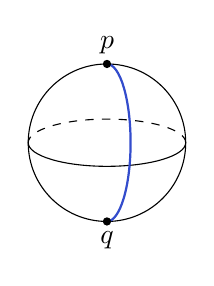
\begin{tikzpicture}
    \draw circle [radius=1];
    \draw [dashed] (1, 0) arc (0:180:1 and 0.3);
    \draw (1, 0) arc (0:-180:1 and 0.3);

    \draw [mblue, thick] (0, 1) arc (90:-90:0.3 and 1);
    \node [circ] at (0, 1) {};
    \node [above] at (0, 1) {$p$};

    \node [circ] at (0, -1) {};
    \node [below] at (0, -1) {$q$};
  \end{tikzpicture}
\end{center}
Then while the geodesic between them does minimize distance, it does not do so strictly.

We also do not guarantee global minimization of length. For example, we can consider the torus
\[
  T^n = \R^n/\Z^n.
\]
This has a flat metric from $\R^n$, and the derivative of the exponential map is the ``identity'' on $\R^n$ at all points. So the geodesics are the straight lines in $\R^n$. Now consider any two $p, q \in T^n$, then there are infinitely many geodesics joining them, but typically, only one of them would be the shortest.

\begin{center}
  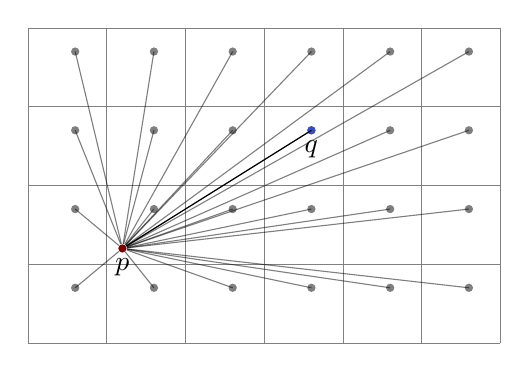
\begin{tikzpicture}
    \draw [step=1cm, gray, very thin] (0, 0) grid (6, 4);

    \node [circ, mred] (p) at (1.2, 1.2) {};
    \node [below] at (p) {$p$};

    \foreach \x in {0,1,2,3,4,5} {
      \foreach \y in {0, 1, 2, 3} {
        \pgfmathsetmacro\a{\x + 0.6}
        \pgfmathsetmacro\b{\y + 0.7}
        \node [circ, opacity=0.5] at (\a, \b) {};
      
        \draw [opacity=0.5] (p) -- (\a, \b);
      }
    }
    \node [circ, mblue] at (3.6, 2.7) {};
    \node [below] at (3.6, 2.7) {$q$};
    \draw (p) -- (3.6, 2.7);
  \end{tikzpicture}
\end{center}

\begin{proof}
  The idea of the proof is that if $\psi$ is any curve close to $\gamma$, then we can use the regularity condition to lift the curve back up to $T_p M$, and then apply our previous result.

  Write $\varphi(t) = ta \in T_p M$. Then by the regularity assumption, for all $t \in [0, 1]$, we know $\exp_p$ is a diffeomorphism of some neighbourhood $W(t)$ of $\varphi(t) = at \in T_p M$ onto the image. By compactness, we can cover $[0, 1]$ by finitely many such covers, say $W(t_1), \cdots, W(t_n)$. We write $W_i = W(t_i)$, and we wlog assume
  \[
    0 = t_0 < t_1 < \cdots < t_k = 1.
  \]
  By cutting things up, we may assume
  \[
    \gamma([t_i, t_{i + 1}]) \subseteq W_i. 
  \]
  We let
  \[
    U = \bigcup \exp_p (W_i).
  \]
  Again by compactness, there is some $\varepsilon < 0$ such that for all $t \in [t_i, t_{i + 1}]$, we have $B(\gamma(t), \varepsilon) \subseteq W_i$.
 
  Now consider any curve $\psi$ of distance $\varepsilon$ away from $\gamma$. Then $\psi([t_i, t_{i + 1}]) \subseteq W_i$. So we can lift it up to $T_p M$, and the end point of the lift is $a$. So we are done by local minimization of length.
\end{proof}
Note that the tricky part of doing the proof is to make sure the lift of $\psi$ has the same end point as $\gamma$ in $T_p M$, which is why we need to do it neighbourhood by neighbourhood.

\subsection{Completeness and the Hopf--Rinow theorem}
There are some natural questions we can ask about geodesics. For example, we might want to know if geodesics can be extended to exist for all time. We might also be interested if distances can always be realized by geodesics. It turns out these questions have the same answer.

\begin{defi}[Geodesically complete]\index{geodesically complete}\index{complete!geodesically}
  We say a manifold $(M, g)$ is \emph{geodesically complete} if each geodesic extends for all time. In other words, for all $p \in M$, $\exp_p$ is defined on \emph{all} of $T_p M$.
\end{defi}

\begin{eg}
  The upper half plane
  \[
    H^2 = \{(x, y) : y> 0\}
  \]
  under the induced Euclidean metric is not geodesically complete. However, $H^2$ and $\R^2$ are diffeomorphic but $\R^2$ is geodesically complete.
\end{eg}

The first theorem we will prove is the following:
\begin{thm}
  Let $(M, g)$ be geodesically complete. Then any two points can be connected by a minimal geodesic.
\end{thm}
In fact, we will prove something stronger --- let $p \in M$, and suppose $\exp_p$ is defined on all of $T_p M$. Then for all $q \in M$, there is a minimal geodesic between them.

To prove this, we need a lemma
\begin{lemma}
  Let $p, q \in M$. Let
  \[
    S_\delta = \{x \in M: d(x, p) = \delta\}.
  \]
  Then for all sufficiently small $\delta$, there exists $p_0 \in S_\delta$ such that
  \[
    d(p, p_0) + d(p_0, q) = d(p, q).
  \]
\end{lemma}
 % insert a picture?
\begin{proof}
  For $\delta > 0$ small, we know $S_\delta = \Sigma_\delta$ is a geodesic sphere about $p$, and is compact. Moreover, $d(\ph, q)$ is a continuous function. So there exists some $p_0 \in \Sigma_\delta$ that minimizes $d(\ph, q)$.

  Consider an arbitrary $\gamma \in \Omega(p, q)$. For the sake of sanity, we assume $\delta < d(p, q)$. Then there is some $t$ such that $\gamma(t) \in \Sigma_\delta$, and
  \[
    \ell(\gamma) \geq d(p, \gamma(t)) + d(\gamma(t), q) \geq d(p, p_0) + d(p_0, q).
  \]
  So we know
  \[
    d(p, q) \geq d(p, p_0) + d(p_0, p).
  \]
  The triangle inequality gives the opposite direction. So we must have equality.
\end{proof}

We can now prove the theorem.
\begin{proof}[Proof of theorem]
  We know $\exp_p$ is defined on $T_p M$. Let $q \in M$. Let $q \in M$. We want a minimal geodesic in $\Omega(p, q)$. By the first lemma, there is some $\delta > 0$ and $p_0$ such that
  \[
    d(p, p_0) = \delta,\quad d(p, p_0) + d(p_0, q) = d(p, q).
  \]
  Also, there is some $v \in T_p M$ such that $\exp_p v = p_0$. We let
  \[
    \gamma_p (t) = \exp_p\left(t \frac{v}{|v|}\right).
  \]
  We let
  \[
    I = \{t \in \R: d(q, \gamma_p(t)) + t = d(p, q)\}.
  \]
  Then we know
  \begin{enumerate}
    \item $\delta \in I$
    \item $I$ is closed by continuity.
  \end{enumerate}
  Let
  \[
    T = \sup\{I \cap [0, d(p, q)]\}.
  \]
  Since $I$ is closed, this is in fact a maximum. So $T \in I$. We claim that $T = d(p, q)$. If so, then $\gamma_p \in \Omega(p, q)$ is the desired minimal geodesic, and we are done.

  Suppose this were not true. Then $T < d(p, q)$. We apply the lemma to $\tilde{p} = \gamma_p(T)$, and $q$ remains as before. Then we can find $\varepsilon > 0$ and some $p_1 \in M$ with the property that
  \begin{align*}
    d(p_1, q) &= d(\gamma_p(T), q) - d(\gamma_p(T), p_1) \\
    &= d(\gamma_p(T), q) - \varepsilon\\
    &= d(p, q) - T - \varepsilon
  \end{align*}
  Hence we have
  \[
    d(p, p_1) \geq d(p, q) - d(q, p_1) = T + \varepsilon.
  \]
  Let $\gamma_1$ be the radial (hence minimal) geodesic from $\gamma_p(T)$ to $p_1$. Now we know
  \[
    \ell(\gamma_p|_{[0, T]}) + \ell(\gamma_1) = T + \varepsilon.
  \]
  So $\gamma_1$ concatenated with $\gamma_p|_{[0, T]}$ is a length-minimizing geodesic from $p$ to $p_1$, and is hence a geodesic. So in fact $p_1$ lies on $\gamma_p$, say $p_1 = \gamma_p(T + s)$ for some $s$. Then $T + s \in I$, which is a contradiction. So we must have $T = d(p, q)$, and hence
  \[
    d(q, \gamma_p(T)) + T = d(p, q),
  \]
  hence $d(q, \gamma_p(T)) = 0$, ie. $q = \gamma_p(T)$.
\end{proof}

\begin{cor}[Hopf--Rinow theorem]\index{Hopf--Rinow theorem}
  For a connected Riemannian manifold $(M, g)$, the following are equivalent:
  \begin{enumerate}
    \item $(M, g)$ is geodesically complete.
    \item For all $p \in M$, $\exp_p$ is defined on all $T_p M$.
    \item For some $p \in M$, $\exp_p$ is defined on all $T_p M$.
    \item Every closed and bounded subset of $(M, d)$ is compact.
    \item $(M, d)$ is complete as a metric space.
  \end{enumerate}
\end{cor}

\begin{proof}
  (i) and (ii) are equivalent by definition. (ii) $\Rightarrow$ (iii) is clear, and we proved (iii) $\Rightarrow$ (ii).

  \begin{itemize}
    \item (iii) $\Rightarrow$ (iv): Let $K \subseteq M$ be closed and bounded. Then by boundedness, $K$ is contained in $\exp_p(\overline{B(0, R)})$. Let $K'$ be the pre-image of $K$ under $\exp_p$. Then it is a closed and bounded subset of $\R^n$, hence compact. Then $K$ is the continuous image of a compact set, hence compact.
    \item (iv) $\Rightarrow$ (v): This is a general topological fact.
    \item (v) $\Rightarrow$ (i): Let $\gamma(t): I \to \R$ be a geodesic, where $I \subseteq \R$. We wlog $|\dot{\gamma}| \equiv 1$. Suppose $I \not= \R$. We wlog $\sup I = a < \infty$. Then $\lim_{t \to a} \gamma(t)$ exist by completeness, and hence $\gamma(a)$ exists. Since geodesics are locally defined near $a$, we can pick a geodesic in the direction of $\lim_{t \to a} \gamma'(t)$. So we can extend $\gamma$ further, which is a contradiction.
  \end{itemize}
\end{proof}

\subsection{Variations of arc length and energy}
This section is mostly a huge computation. As we previously saw, geodesics are locally length-minimizing, and we shall see that another quantity, namely the energy is also a useful thing to consider, as minimizing the energy also forces the parametrization to be constant speed.

To make good use of these properties of geodesics, it is helpful to compute explicitly expressions for how length and energy change along variations. The computations are largely uninteresting, but it will pay off.

\begin{defi}[Energy]\index{energy}
  The \emph{energy function} $E: \Omega(p, q) \to \R$ is given by
  \[
    E(\gamma) = \frac{1}{2} \int_0^T|\dot{\gamma}|^2\;\d t,
  \]
  where $\gamma: [0, T] \to M$.
\end{defi}
Recall that $\Omega(p, q)$ is defined as the space of piecewise $C^1$ curves. Often, we will make the simplifying assumption that all curves are in fact $C^1$. It doesn't really matter.

Note that the length of a curve is independent of parametrization. Thus, if we are interested in critical points, then the critical points cannot possibly be isolated, as we can just re-parametrize to get a nearby path with the same length. On the other hand, the energy $E$ \emph{does} depend on parametrization. This does have isolated critical points, which is technically very convenient.

\begin{prop}
  Let $\gamma_0: [0, T] \to M$ be a path from $p$ to $q$ such that for all $\gamma \in \Omega(p, q)$ with $\gamma:[0, T] \to M$, we have $E(\gamma) \geq E(\gamma_0)$. Then $\gamma_0$ must be a geodesic.
\end{prop}

Recall that we already had such a result for length instead of energy. The proof is just the application of Cauchy-Schwartz.

\begin{proof}
  By the Cauchy-Schwartz inequality, we have
  \[
    \int_0^T |\dot{\gamma}|^2\; \d t \geq \left(\int_0^T |\dot{\gamma}(t)|\;\d t\right)^2
  \]
  with equality iff $|\dot{\gamma}|$ is constant. In other words,
  \[
    E(\gamma) \geq \frac{\ell(\gamma)^2}{2T}.
  \]
  So we know that if $\gamma_0$ minimizes energy, then it must be constant speed. Now given any $\gamma$, if we just care about its length, then we may wlog it is constant speed, and then
  \[
    \ell(\gamma) = \sqrt{2E(\gamma)T }\geq \sqrt{2 E(\gamma_0)T} = \ell(\gamma_0).
  \]
  So $\gamma_0$ minimizes length, and thus $\gamma_0$ is a geodesic.
\end{proof}

We shall consider smooth variations $H(t, s)$ of $\gamma_0(t) = H(t, 0)$. We require that $H: [0, T] \times (-\varepsilon, \varepsilon) \to M$ is smooth. Since we are mostly just interested in what happens ``near'' $s = 0$, it is often convenient to just consider the corresponding vector field along $\gamma$:
\[
  Y(t) = \left.\frac{\partial H}{\partial s}\right|_{s = 0} = (\d H)_{(t, 0)} \frac{\partial}{\partial s},
\]
Conversely, given any such vector field $Y$, we can generate a variation $H$ that gives rise to $Y$. For example, we can put
\[
  H(t, s) = \exp_{\gamma_0(t)} (sY(t)),
\]
which is valid on some neighbourhood of $[0, T] \times \{0\}$. If $Y(0) = 0 = Y(T)$, then we can choose $H$ fixing end-points of $\gamma_0$.

\begin{thm}[First variation formula]\index{first variation formula!geodesic}\index{geodesic!first variation formula}\leavevmode
  \begin{enumerate}
    \item For any variation $H$ of $\gamma$, we have
      \[
        \left.\frac{\d}{\d s}E(\gamma_s)\right|_{s = 0} = g(Y(t), \dot{\gamma}(t))|_0^T - \int_0^T g\left(Y(t), \frac{\nabla}{\d t} \dot{\gamma}(t)\right)\;\d t.\tag{$*$}
      \]
    \item The critical points, ie. the $\gamma$ such that
      \[
        \left.\frac{\d}{\d s} E(\gamma_s)\right|_{s = 0}
      \]
      for all (end-point fixing) variation $H$ of $\gamma$, are geodesics.
    \item If $|\dot{\gamma}_s(t)|$ is constant for each fixed $s \in (-\varepsilon, \varepsilon)$, and $|\dot{\gamma}(t)| \equiv 1$, then
      \[
        \left.\frac{\d}{\d s}E(\gamma_s) \right|_{s = 0} = \left.\frac{\d}{\d s} \ell(\gamma_s)\right|_{s = 0}
      \]
    \item If $\gamma$ is a critical point of the length, then it must be a reparametrization of a geodesic.
  \end{enumerate}
\end{thm}
This is just some calculations.

\begin{proof}
  We will assume that we can treat $\frac{\partial}{\partial s}$ and $\frac{\partial}{\partial t}$ as vector fields on an embedded submanifold, even though $H$ is not necessarily a local embedding.

  The result can be proved without this assumption, but will require more technical work.
  \begin{enumerate}
    \item We have
      \begin{align*}
        \frac{1}{2} \frac{\partial}{\partial s} g(\dot{\gamma}_s(t), \dot{\gamma}_s(t)) &= g\left(\frac{\nabla}{\d s} \dot{\gamma}_s(t), \dot{\gamma}_s(t)\right)\\
        &= g\left(\frac{\nabla}{\d t} \frac{\partial H}{\partial s}(t, s), \frac{\partial H}{\partial t} (t, s)\right)\\
        &= \frac{\partial}{\partial t} g\left(\frac{\partial H}{\partial s}, \frac{\partial H}{\partial t}\right) - g \left(\frac{\partial H}{\partial s}, \frac{\nabla}{\d t} \frac{\partial H}{\partial t}\right).
      \end{align*}
      Comparing with what we want to prove, we see that we get what we want by integrating $\int_0^T\;\d t$, and then putting $s = 0$, and then noting that
      \[
        \left.\frac{\partial H}{\partial s}\right|_{s = 0} = Y,\quad \left.\frac{\partial H}{\partial t}\right|_{s = 0} = \dot{\gamma}.
      \]
    \item If $\gamma$ is a geodesic, then
      \[
        \frac{\nabla}{\d t} \dot{\gamma}(t) = 0.
      \]
      So the integral on the right hand side of $(*)$ vanishes. Also, we have $Y(0) = 0 = Y(T)$. So the RHS vanishes.

      Conversely, suppose $\gamma$ is a critical point for $E$. Then choose $H$ with
      \[
        Y(t) = f(t) \frac{\nabla}{\d t} \dot{\gamma}(t)
      \]
      for some $f \in C^\infty[0, T]$ such that $f(0) = f(T) = 0$. Then we know
      \[
        \int_0^T f(t) \left|\frac{\nabla}{\d t} \dot{\gamma}(t)\right|^2 \;\d t = 0,
      \]
      and this is true for all $f$. So we know
      \[
        \frac{\nabla}{\d t}\dot{\gamma} = 0.
      \]
    \item This is evident from the previous proposition. Indeed, we fix $[0, T]$, then for all $H$, we have
      \[
        E(\gamma_s) = \frac{\ell (\gamma_s)^2}{2T},
      \]
      and so
      \[
        \left.\frac{\d}{\d s} E(\gamma_s)\right|_{s = 0} = \frac{1}{T} \ell(\gamma_s) \left.\frac{\d}{\d s}\ell(\gamma_s) \right|_{s = 0},
      \]
     and when $s = 0$, the curve is parametrized by arc-length, so $\ell(\gamma_s) = T$.
   \item By reparametrization, we may wlog $|\dot{\gamma}| \equiv 1$. Then $\gamma$ is a critical point for $\ell$, hence for $E$, hence a geodesic.
  \end{enumerate}
\end{proof}
Often, we are interested in more than just whether the curve is a critical point. We want to know if it maximizes or minimizes energy. Then we need more than the ``first derivative''. We need the ``second derivative'' as well.

\begin{thm}[Second variation formula]\index{second variation formula!geodesic}\index{geodesic!second variation formula}\leavevmode
  Let $\gamma(t): [0, T] \to M$ be a geodesic with $|\dot{\gamma}| = 1$. Let $H(t, s)$ be a variation of $\gamma$. Let
  \[
    Y(t, s) = \frac{\partial H}{\partial s}(t, s) =  (\d H)_{(t, s)} \frac{\partial}{\partial s}.
  \]
  Then
  \begin{enumerate}
    \item We have
      \[
        \left.\frac{\d^2}{\d s^2} E(\gamma_s)\right|_{s = 0} = \left.g\left(\frac{\nabla Y}{\d s}(t, 0), \dot{\gamma}\right)\right|_0^T + \int_0^T (|Y'|^2 - R(Y, \dot\gamma, Y, \dot{\gamma})) \;\d t.
      \]
    \item Also
      \begin{multline*}
        \left.\frac{\d^2}{\d s^2}\ell(\gamma_s)\right|_{s = 0} = \left.g\left(\frac{\nabla Y}{\d s} (t, 0), \dot{\gamma}(t)\right)\right|_0^T \\
        + \int_0^T \left( |Y'|^2 - R(Y, \dot{\gamma}, Y, \dot{\gamma}) - g(\dot{\gamma}, Y')^2\right)\;\d t,
      \end{multline*}
      where $R$ is the $(4, 0)$ curvature tensor, and
      \[
        Y'(t) = \frac{\nabla Y}{\d t}(t, 0).
      \]
      Putting
      \[
        Y_n = Y - g(Y, \dot{\gamma}) \dot{\gamma}
      \]
      for the normal component of $Y$, we can write this as
      \[
        \left.\frac{\d^2}{\d s^2}\ell(\gamma_s)\right|_{s = 0} = \left.g\left(\frac{\nabla Y_n}{\d s} (t, 0), \dot{\gamma}(t)\right)\right|_0^T + \int_0^T \left( |Y'_n|^2 - R(Y_n, \dot{\gamma}, Y_n, \dot{\gamma})\right)\;\d t.
      \]
  \end{enumerate}
\end{thm}
Note that if we have fixed end points, then the first terms in the variation formulae vanish.

\begin{proof}
  We use
  \[
    \frac{\d}{\d s}E(\gamma_s) = \left.g(Y(t, s), \dot{\gamma}_s(t))\right|_{t = 0}^{t = T} - \int_0^T g\left(Y(t, s), \frac{\nabla}{\d t} \dot{\gamma}_s(t)\right)\;\d t.
  \]
  Taking the derivative with respect to $s$ again gives
  \begin{multline*}
    \frac{\d^2}{\d s^2}E(\gamma_s) =\left. g\left(\frac{\nabla Y}{\d s}, \dot{\gamma}\right)\right|_{t = 0}^{t = T} + \left.g\left(Y, \frac{\nabla}{\d s} \dot{\gamma}_s\right)\right|_{t = 0}^{T} \\
    - \int_0^T \left(g\left(\frac{\nabla Y}{\d s}, \frac{\nabla}{\d t} \dot{\gamma}_s\right) + g\left(Y, \frac{\nabla}{\d s} \frac{\nabla}{\d t} \dot{\gamma}\right)\right)\;\d t.
  \end{multline*}
  We now use that
  \begin{align*}
    \frac{\nabla}{\d s} \frac{\nabla}{\d t} \dot\gamma_s(t) &= \frac{\nabla}{\d t} \frac{\nabla}{\d s} \dot{\gamma}_s(t) + R\left(\frac{\partial H}{\partial s}, \frac{\partial H}{\partial t}\right)\dot{\gamma}_s\\
    &= \left(\frac{\nabla}{\d t}\right)^2 Y(t, s) + R\left(\frac{\partial H}{\partial s}, \frac{\partial H}{\partial t}\right)\dot{\gamma}_s.
  \end{align*}
  We now set $s = 0$, and then the above gives
  \begin{multline*}
    \left.\frac{\d^2}{\d s^2} E(\gamma_s)\right|_{s = 0} = \left.g\left(\frac{\nabla Y}{\d s}, \dot{\gamma}\right)\right|_0^T + \left.g\left(Y, \frac{\nabla \dot{\gamma}}{\d s}\right)\right|_0^T \\
    - \int_0^T \left[g\left(Y, \left(\frac{\nabla}{\d t}\right)^2 Y\right) + R(\dot{\gamma}, Y, \dot{\gamma}, Y)\right]\;\d t.
  \end{multline*}
  Finally, applying integration by parts, we can write
  \[
    -\int_0^T g\left(Y, \left(\frac{\nabla}{\d t}\right)^2 Y\right) \;\d t= - \left.g\left(Y, \frac{\nabla}{\d t}Y\right)\right|_0^T + \int_0^T \left|\frac{\nabla Y}{\d t}\right|^2\;\d t.
  \]
  Finally, noting that
  \[
    \frac{\nabla}{\d s} \dot{\gamma}(s) = \frac{\nabla}{\d t} Y(t, s),
  \]
  we find that
  \[
    \left.\frac{\d^2}{\d s^2} E(\gamma_s)\right|_{s = 0} = \left.g\left(\frac{\nabla Y}{\d s}, \dot{\gamma}\right)\right|_0^T + \int_0^T \left(|Y'|^2 - R(Y, \dot{\gamma}, Y, \dot{\gamma})\right)\;\d t.
  \]
  It remains to prove the second variation of length. We first differentiate
  \[
    \frac{\d}{\d s}\ell(\gamma_s) = \int_0^T \frac{1}{2 \sqrt{g(\dot{\gamma}_s, \dot{\gamma}_s)}} \frac{\partial}{\partial s} g(\dot{\gamma}_s, \dot{\gamma}_s)\;\d t.
  \]
  Then the second derivative gives
  \[
    \left.\frac{\d^2}{\d s^2} \ell(\gamma_s) \right|_{s = 0} = \int_0^T \left[\frac{1}{2} \left.\frac{\partial^2}{\partial s^2} g(\dot{\gamma}_s, \dot{\gamma}_s) \right|_{s = 0} - \left.\frac{1}{4} \left(\frac{\partial}{\partial s} g(\dot{\gamma}_s, \dot{\gamma}_s)\right)^2\right|_{s = 0}\right]\;\d t,
  \]
  where we used the fact that $g(\dot{\gamma}, \dot{\gamma}) = 1$.

  We notice that the first term can be identified with the derivative of the energy function. So we have
  \[
    \left.\frac{\d^2}{\d s^2} \ell(\gamma_s) \right|_{s = 0} = \left.\frac{\d^2}{\d s^2} E(\gamma_s)\right|_{s = 0} - \int_0^T \left( \left.g\left(\dot{\gamma}_s, \frac{\nabla}{\d s} \dot{\gamma}_s\right)\right|_{s = 0}\right)^2\;\d t.
  \]
  So the second part follows from the first.
\end{proof}

\subsection{Applications}
This finally puts us in a position to prove something more interesting.

\subsubsection*{Synge's theorem}
We are first going to prove the following remarkable result relating curvature and topology:
\begin{thm}[Synge's theorem]\index{Synge's theorem}
  Every compact orientable Riemannian manifold $(M, g)$ such that $\dim M$ is even and has $K(g) > 0$ for all planes at $p \in M$ is simply connected.
\end{thm}

We can see that these conditions are indeed necessary. For example, we can consider $\RP^2 = S^2/\pm 1$ with the induced metric from $S^2$. Then this is compact with positive sectional curvature, but it is not orientable. Indeed it is not simply connected.

Similarly, if we take $\RP^3$, then this has odd dimension, and the theorem breaks.

Finally, we do need strict inequality, eg. the flat torus is not simply connected.

We first prove a technical lemma.
\begin{lemma}
  Let $M$ be a compact manifold, and $[\alpha]$ a non-trivial homotopy class of closed curves in $M$. Then there is a closed minimal geodesic in $[\alpha]$.
\end{lemma}

\begin{proof}
  Since $M$ is compact, we can pick some $\varepsilon > 0$ such that for all $p \in M$, the map $\exp_p |_{B(0, p)}$ is a diffeomorphism.

  Let $\ell = \inf_{\gamma \in [\alpha]} \ell(\gamma)$. We know that $\ell > 0$, otherwise, there exists a $\gamma$ with $\ell(\gamma) < \varepsilon$. So $\gamma$ is contained in some geodesic coordinate neighbourhood, but then $\alpha$ is contractible. So $\ell$ must be positive.

  Then we can find a sequence $\gamma_n \in [\alpha]$ with $\gamma_n: [0, 1] \to M$, $|\dot{\gamma}|$ constant, such that
  \[
    \lim_{n \to \infty} \ell(\gamma_n) = \ell.
  \]
  Choose
  \[
    0 = t_0 < t_1 < \cdots < t_k = 1
  \]
  such that
  \[
    t_{i + 1} - t_i < \frac{\varepsilon}{2 \ell}.
  \]
  So it follows that
  \[
    d(\gamma_n(t_i), \gamma_n(t_{i + 1})) < \varepsilon
  \]
  for all $n$ sufficiently large and all $i$. Then again, we can replace $\gamma_n|_{[t_i, t_{i + 1}]}$ by a radial geodesic without affecting the limit $\lim \ell(\gamma_n)$.

  Then we exploit the compactness of $M$ (and the unit sphere) again, and pass to a subsequence of $\{\gamma_n\}$ so that $\gamma_n(t_i), \dot{\gamma}_n (t_i)$ are all convergent for every fixed $i$ as $n \to \infty$. Then the curves converges to some
  \[
    \gamma_n \to \hat{\gamma} \in [\alpha],
  \]
  given by joining the limits $\lim_{n \to \infty} \gamma_n(t_i)$. Then we know that the length converges as well, and so we know $\hat{\gamma}$ is minimal among curves in $[\alpha]$. So $\hat{\gamma}$ is locally minimal, hence a geodesic. So we can take $\gamma = \hat{\gamma}$, and we are done.
\end{proof}

\begin{proof}[Proof of Synge's theorem]
  Suppose $M$ satisfies the hypothesis, but $\pi_1(M) \not= \{1\}$. So there is a path $\alpha$ with $[\alpha] \not= 1$, ie. it cannot be contracted to a point. By the lemma, we pick a representative $\gamma$ of $[\alpha]$ that is a closed, minimal geodesic.

  We now prove the theorem. We may wlog assume $|\dot{\gamma}| = 1$, and $t$ ranges in $[0, T]$. Consider a vector field $X(t)$ for $0 \leq t \leq T$ along $\gamma(t)$ such that
  \[
    \frac{\nabla X}{\d t} = 0,\quad g(X(0), \dot{\gamma}(0)) = 0.
  \]
  Note that since $g$ is a geodesic, we know
  \[
    g(X(t), \dot{\gamma}(t)) = 0,
  \]
  for all $t \in [0, T]$ as parallel transport preserves the inner product. So $X(T) \perp \dot{\gamma}(T) = \dot{\gamma}(0)$ since we have a closed curve.

  We consider the map $P$ that sends $X(0) \mapsto X(T)$. This is a linear isometry of $(\dot{\gamma}(0))^\perp$ with itself that preserves orientation. So we can think of $P$ as a map
  \[
    P \in \SO(2n - 1),
  \]
  where $\dim M = 2n$. It is an easy linear algebra exercise to show that every element of $\SO(2n - 1)$ must have an eigenvector of eigenvalue $1$. So we can find $v \in T_p M$ such that $v \perp \dot{\gamma}(0)$ and $P(v) = v$. We take $X(0) = v$. Then we have $X(T) = v$.

  Consider now a variation $H(t, s)$ inducing this $X(t)$. We may assume $|\dot{\gamma}_s|$ is constant. Then
  \[
    \frac{\d}{\d s} \ell(\gamma_s)|_{s = 0} = 0
  \]
  as $\gamma$ is minimal. Moreover, since it is a minimum, the second derivative must be positive, or at least non-negative. Is this actually the case? 
  
  We look at the second variation formula of length. Using the fact that the loop is closed, the formula reduces to
  \[
    \left.\frac{\d^2}{\d s^2} \ell(\gamma_s)\right|_{s = 0} = - \int_0^T R(X, \dot{\gamma}, X, \dot{\gamma})\;\d t.
  \]
  But we assumed the sectional curvature is positive. So the second variation is negative! This is a contradiction.
\end{proof}

\subsubsection*{Conjugate points}
Recall that when a geodesic starts moving, for a short period of time, it is length-minimizing. However, in general, if we keep on moving for a long time, then we cease to be minimizing. The point where this transition happens is interesting.

As before, for a vector field $J$ along a curve $\gamma(t)$, we will write
\[
  J' = \frac{\nabla J}{\d t}.
\]
\begin{defi}[Conjugate points]\index{conjugate points}
  Let $\gamma(t)$ be a geodesic. Then
  \[
    p = \gamma(\alpha), \quad q = \gamma(\beta)
  \]
  are \emph{conjugate points} if there exists some non-trivial $J$ such that $J(\alpha) = 0 = J(\beta)$.
\end{defi}
It is easy to see that this does not depend on parametrization of the curve, because Jacobi fields do not.

\begin{prop}\leavevmode
  \begin{enumerate}
    \item If $\gamma(t) = \exp_p(t a)$ and $q = \exp_p(\beta a)$ is conjugate to $p$, then $q$ is a singular value of $\exp$.
    \item Let $J$ be as in the definition. Then $J$ must be pointwise normal to $\dot{\gamma}$.
  \end{enumerate}
\end{prop}

\begin{proof}\leavevmode
  \begin{enumerate}
    \item We wlog $[\alpha, \beta] = [0, 1]$. So $J(0) = 0 = J(1)$. We $a = \dot{\gamma}(0)$ and $w = J'(0)$. Note that $a, w$ are both non-zero, as Jacobi fields are determined by initial conditions. Then $q = \exp_p(a)$.

      We have shown earlier that if $J(0) = 0$, then
      \[
        J(t) = (\d \exp_p)_{ta} (tw)
      \]
      for all $0 \leq t \leq 1$. So it follows $(\d \exp_p)_{a}(w) = J(1) = 0$. So $(\d \exp_p)_a$ has non-trivial kernel, and hence isn't surjective.
    \item We claim that any Jacobi field $J$ along a geodesic $\gamma$ satisfies
        \[
          g(J(t), \dot{\gamma}(t)) = g(J'(0), \dot{\gamma}(0)) t + g(J(0), \dot{\gamma}(0)).
        \]
      To prove this, we note that by the definition of geodesic and Jacobi fields, we have
      \[
        \frac{\d}{\d t} g(J', \dot{\gamma}) = g(J'', \dot{\gamma}(0)) = -g(R(\dot{\gamma}, J), \dot{\gamma}, \dot{\gamma}) = 0
      \]
      by symmetries of $R$. So we have
      \[
        \frac{\d}{\d t}(J, \dot{\gamma}) = g(J'(t), \dot{\gamma}(t)) = g(J'(0), \dot{\gamma}(0)).
      \]
      Now integrating gives the desired result.

     This result tells us $g(J(t), \dot{\gamma}(t))$ is a linear function of $t$. But we have
      \[
        g(J(0), \dot{\gamma}(0)) = g(J(1), \dot{\gamma}(1)) = 0.
      \]
      So we know $g(J(t), \dot{\gamma}(t))$ is constantly zero.
  \end{enumerate}
\end{proof}
From the proof, we see that for any Jacobi field with $J(0) = 0$, we have
\[
  g(J'(0), \dot{\gamma}(0)) = 0 \Longleftrightarrow g(J(t), \dot{\gamma}(t)) = \text{constant}.
\]
This implies that the dimension of the normal Jacobi fields along $\gamma$ satisfying $J(0) = 0$ is $\dim M - 1$.

\begin{eg}
  Consider $M = S^2 \subseteq \R^3$ with the round metric, ie. the ``obvious'' metric induced from $\R^3$. We claim that $N = (0, 0, 1)$ and $S = (0, 1, 0)$ are conjugate points.

  To construct a Jacobi field, instead of trying to mess with the Jacobi equation, we construct a variation by geodesics. We let
  \[
    f(t, s) = 
    \begin{pmatrix}
      \cos s \sin t\\
      \sin s \sin t\\
      \cos t
    \end{pmatrix}.
  \]
  We see that when $s = 0$, this is the great-circle in the $(x, z)$-plane. Then we have a Jacobi field
  \[
    J(t) = \left.\frac{\partial f}{\partial s}\right|_{s = 0} =
    \begin{pmatrix}
      0\\
      \sin t\\
      0
    \end{pmatrix}.
  \]
  This is then a Jacobi field that vanishes at $N$ and $S$.
  \begin{center}
    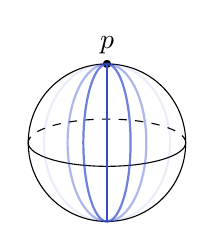
\begin{tikzpicture}
      \draw circle [radius=1];
      \draw [dashed] (1, 0) arc (0:180:1 and 0.3);
      \draw (1, 0) arc (0:-180:1 and 0.3);

      \node [circ] at (0, 1) {};
      \node [above] at (0, 1) {$p$};

      \draw [mblue, thick] (0, 1) arc(90:-90: 0.0 and 1);
      \draw [mblue, opacity=0.7, thick] (0, 1) arc(90:-90: 0.3 and 1);
      \draw [mblue, opacity=0.4, thick] (0, 1) arc(90:-90: 0.5 and 1);
      \draw [mblue, opacity=0.1, thick] (0, 1) arc(90:-90: 0.8 and 1);
      \draw [mblue, opacity=0.7, thick] (0, 1) arc(90:270: 0.3 and 1);
      \draw [mblue, opacity=0.4, thick] (0, 1) arc(90:270: 0.5 and 1);
      \draw [mblue, opacity=0.1, thick] (0, 1) arc(90:270: 0.8 and 1);
    \end{tikzpicture}
  \end{center}
\end{eg}
When we are \emph{at} the conjugate point, then there are many adjacent curves whose length is equal to ours. If we extend our geodesic \emph{beyond} the conjugate point, then it is no longer even locally minimal:
\begin{center}
  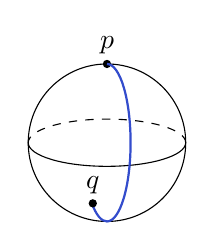
\begin{tikzpicture}
    \draw circle [radius=1];
    \draw [dashed] (1, 0) arc (0:180:1 and 0.3);
    \draw (1, 0) arc (0:-180:1 and 0.3);

    \node [circ] at (0, 1) {};
    \node [above] at (0, 1) {$p$};

    \draw [mblue, thick] (0, 1) arc(90:-130: 0.3 and 1);

    \node [circ] (q) at (-0.18, -0.77) {};
    \node [above] at (q) {$q$};
  \end{tikzpicture}
\end{center}
We can push the geodesic slightly over and the length will be shorter. On the other hand, we proved that up to the conjugate point, the geodesic is always locally minimal.

In turns out this phenomenon is generic:

\begin{thm}
  Let $\gamma: [0, 1] \to M$ be a geodesic with $\gamma(0) = p$, $\gamma(1) = q$ such that $p$ is conjugate to some $\gamma(t_0)$ for some $t_0 \in (0, 1)$. Then there is a piecewise smooth variation of $f(t, s)$ with $f(t, 0) = \gamma(t)$ such that
  \[
    f(0, s) = p,\quad f(1, s) = q
  \]
  and $\ell(f(\ph, s)) < \ell(\gamma)$ whenever $s \not= 0$ is small.
\end{thm}

The proof is a generalization of the example we had above. We know that up to the conjugate point, we have a Jacobi filed that allows us to vary the geodesic without increasing the length. We can then give it a slight ``kick'' and then the length will decrease.

\begin{proof}
  By the hypothesis, there is a $J(t)$ defined on $t \in [0, 1]$ and $t_0 \in (0, 1)$ such that
  \[
    J(t) \perp \dot{\gamma}(t)
  \]
  for all $t$, and $J(0) = J(t_0) = 0$ and $J \not\equiv 0$. Then $J'(t_0) \not= 0$.

  We define a parallel vector field $Z_1$ along $\gamma$ by $Z_1(t_0) = -J'(t_0)$. We pick $\theta \in C^\infty[0, 1]$ such that $\theta(0) = \theta(1) = 0$ and $\theta(t_0) = 1$.

  Finally, we define
  \[
    Z = \theta Z_1,
  \]
  and for $\alpha \in \R$, we define
  \[
    Y_\alpha(t) =
    \begin{cases}
      J(t) + \alpha Z(t) & 0 \leq t \leq t_0\\
      \alpha Z(t) & t_0 \leq t \leq 1
    \end{cases}.
  \]
  We notice that this is not smooth at $t_0$, but is just continuous. We will postpone the choice of $\alpha$ to a later time.

  We know $Y_\alpha(t)$ arises from a piecewise $C^\infty$ variation of $\gamma$, say $H_\alpha(t, s)$. The technical claim is that the second variation of length corresponding to $Y_\alpha(t)$ is negative for some $\alpha$.

  We denote by $I(X, Y)_T$ the symmetric bilinear form that gives rise to the second variation of length with fixed end points. If we make the additional assumption that $X, Y$ are normal along $\gamma$, then the formula simplifies, and reduces to
  \[
    I(X, Y)_T = \int_0^T \left(g(X', Y') - R(X, \dot{\gamma}, Y, \dot{\gamma})\right)\;\d t.
  \]
  Then for $H_\alpha(t, s)$, we have
  \begin{align*}
    \left.\frac{\d^2}{\d s^2}\ell(\gamma_s)\right|_{s = 0} &= I_1 + I_2 + I_3\\
    I_1 &= I(J, J)_{t_0}\\
    I_2 &= 2\alpha I(J, Z)_{t_0}\\
    I_3 &= \alpha^2 I(Z, Z)_1.
  \end{align*}
  We look at each term separately.

  We first claim that $I_1 = 0$. We note that
  \[
    \frac{\d}{\d t} g(J, J') = g(J', J') + g(J, J''),
  \]
  and $g(J, J'')$ added to the curvature vanishes by the Jacobi equation. Then by integrating by parts and applying the boundary condition, we see that $I_1$ vanishes.

  Also, by integrating by parts, we find
  \[
    I_2 = \left. 2 \alpha g(Z, J') \right|_0^{t_0}.
  \]
  Whence
  \[
    \left.\frac{\d^2}{\d s^2}\ell(\gamma_s)\right|_{s = 0} = -2\alpha |J'(t_0)|^2 + \alpha^2 I(Z, Z)_1.
  \]
  Now if $\alpha > 0$ is very very small, then the linear term dominates, and this is negative. Since the first variation vanishes ($\gamma$ is a geodesic), we know this is a local maximum of length.
\end{proof}
Note that we made a compromise in the theorem by doing a piecewise $C^\infty$ variation instead of a smooth one, but of course, we can fix this by making a smooth approximation.

\subsubsection*{Bonnet--Myers diameter theorem}
We are going to see yet another application of our previous hard work, which may also be seen as an interplay between curvature topology. In case it isn't clear, all our manifolds are connected.

\begin{defi}[Diameter]\index{diameter}
  The \emph{diameter} of a Riemannian manifold $(M, g)$ is
  \[
    \diam(M, g) = \sup_{p, q \in M} d(p, q).
  \]
\end{defi}
Of course, this definition is valid for any metric space.
\begin{eg}
  Consider the sphere
  \[
    S^{n - 1}(r) = \{x \in \R^n: |x| = r\},
  \]
  with the induced ``round'' metric. Then
  \[
    \diam (S^{n - 1} (r)) = \pi r.
  \]
  It is an exercise to check that
  \[
    K \equiv \frac{1}{r^2}.
  \]
\end{eg}

We will also need the following notation:
\begin{notation}
  Let $h, \hat{h}$ be two symmetric bilinear forms on a real vector space. We say $h \geq \hat{h}$ if $h - \hat{h}$ is non-negative definite.

  If $h, \hat{h} \in \Gamma(S^2 T^* M)$ are fields of symmetric bilinear forms, we write $h \geq \hat{h}$ if $h_p \geq \hat{h}_p$ for all $p \in M$.
\end{notation}

The following will also be useful:
\begin{defi}[Riemannian covering map]\index{Riemannian covering map}\index{covering map!Riemannian}\index{Riemannian covering}\index{Riemannian cover}\index{cover!Riemannian}
  Let $(M, g)$ and $(\tilde{M}, \tilde{g})$ be two Riemannian manifolds, and $f: \tilde{M} \to M$ be a smooth covering map. We say $f$ is a \emph{Riemannian covering map} if it is a local isometry. Alternatively, $f^* g = \tilde{g}$. We say $\tilde{M}$ is a Riemannian cover of $M$.
\end{defi}

Recall that if $f$ is in fact a universal cover, ie. $\tilde{M}$ is simply connected, then we can (non-canonically) identify $\pi_1(M)$ with $f^{-1}(p)$ for any point $p \in M$.

\begin{defi}[Bonnet--Myers diameter theorem]\index{Bonnet--Myers theorem}
  Let $(M, g)$ be a complete $n$-dimensional manifold with
  \[
    \Ric(g) \geq \frac{n - 1}{r^2} g,
  \]
  where $r > 0$ is some positive number. Then
  \[
    \diam(M, g) \leq \diam S^n(r) = \pi r.
  \]
  In particular, $M$ is compact and $\pi_1(M)$ is finite.
\end{defi}

\begin{proof}
  Consider any $L < \diam (M, g)$. Then by definition (and Hopf--Rinow), we can find $p, q \in M$ such that $d(p, q) = L$, and a minimal geodesic $\gamma \in \Omega(p, q)$ with $\ell(\gamma) = d(p, q)$. We parametrize $\gamma: [0, L] \to M$ so that $|\dot{\gamma}| = 1$.

  Now consider any vector field $Y$ along $\gamma$ such that $Y(p) = 0 = Y(q)$. Since $\Gamma$ is a minimal geodesic, it is a critical point for $\ell$, and the second variation $I(Y, Y)_{[0, L]}$ is non-negative (recall that the second variation has fixed end points).

  We extend $\dot{\gamma}(0)$ to an orthonormal basis of $T_p M$, say $\dot{\gamma}(0) = e_1, e_2, \cdots, e_n$. We further let $X_i$ be the unique vector field such that
  \[
    X_i' = 0,\quad X_i(0) = e_i.
  \]
  In particular, $X_1(t) = \dot{\gamma}(t)$.

  For $i = 2, \cdots, n$, we put
  \[
    Y_i(t) = \sin \left(\frac{\pi t}{L}\right) X_i(t).
  \]
  Then after integrating by parts, we find that we have
  \begin{align*}
    I(Y_i, Y_i)_{[0,L]} &= - \int_0^L g(Y_i'' + R(\dot{\gamma}, Y_i) Y_i, \dot{\gamma}) \;\d t\\
    \intertext{Using the fact that $X_i$ is parallel, this can be written as}
    &= \int_0^L \sin^2 \frac{\pi t}{L} \left(\frac{\pi^2}{L^2} - R(\dot{\gamma}, X_i, \dot{\gamma}, X_i)\right)\;\d t,
  \end{align*}
  and since this is length minimizing, we know this is $\geq 0$.

  We note that we have $R(\dot{\gamma}, X_1, \dot{\gamma}, X_1) = 0$. So we have
  \[
    \sum_{i = 2}^n R(\dot{\gamma}, X_i, \dot{\gamma}, X_i) = \Ric(\dot{\gamma}, \dot{\gamma}).
  \]
  So we know
  \[
    \sum_{i = 2}^n I(Y_i, Y_i) = \int_0^L \sin^2 \frac{\pi t}{L}\left((n - 1) \frac{\pi^2}{L} - \Ric(\dot{\gamma}, \dot{\gamma})\right)\;\d t \geq 0.
  \]
  We also know that
  \[
    \Ric(\dot{\gamma}, \dot{\gamma}) \geq \frac{n - 1}{r^2}
  \]
  by hypothesis. So this implies that
  \[
    \frac{\pi^2}{L^2} \geq \frac{1}{r^2}.
  \]
  This tells us that
  \[
    L \leq \pi r.
  \]
  Since $L$ is any number less that $\diam(M, g)$, it follows that
  \[
    \diam(M, g) \leq \pi r.
  \]
  Since $M$ is known to be complete, by Hopf-Rinow theorem, any closed bounded subset is compact. But $M$ itself is closed and bounded! So $M$ is compact.

  To understand the fundamental, group, we simply have to consider a universal Riemannian cover $f: \tilde{M} \to M$. We know such a topological universal covering space must exist by general existence theorems. We can then pull back the differential structure and metric along $f$, since $f$ is a local homeomorphism. So this gives a universal Riemannian cover of $M$. But they hypothesis of the theorem is local, so it is also satisfied for $\tilde{M}$. So it is also compact. Since $f^{-1}(p)$ is a closed discrete subset of a compact space, it is finite, and we are done.
\end{proof}
It is an easy exercise to show that the hypothesis on the Ricci curvature cannot be weakened to just saying that the Ricci curvature is positive definite.

\subsubsection*{Hadamard--Cartan theorem}
To prove the next result, we need to talk a bit more about coverings.
\begin{prop}
  Let $(M, g)$ and $(N, h)$ be Riemannian manifolds, and suppose $M$ is complete. Suppose there is a smooth surjection $f: M \to N$ that is a local diffeomorphism. Moreover, suppose that for any $p \in M$ and $v \in T_p M$, we have $|\d f_p (v)|_h \geq |v|$. Then $f$ is a covering map.
\end{prop}

\begin{proof}
  By general topology, it suffices to prove that for any smooth curve $\gamma: [0, 1] \to N$, and any $q \in M$ such that $f(q) = \gamma(0)$, there exists a lift of $\gamma$ starting from from $q$.
  \[
    \begin{tikzcd}
      & M \ar[d, "f"]\\
      \lbrack 0, 1\rbrack \ar[r, "\gamma"] \ar[ur, dashed, "\tilde{\gamma}"] & N
    \end{tikzcd}
  \]
  From the hypothesis, we know that $\tilde{\gamma}$ exists on $[0, \varepsilon_0]$ for some ``small'' $\varepsilon_0 > 0$. We let
  \[
    I = \{0 \leq \varepsilon \leq : \tilde{\gamma} \text{ exists on }[0, \varepsilon]\}.
  \]
  We immediately see this is non-empty, since it contains $\varepsilon_0$. Moreover, it is not difficult to see that $I$ is open in $[0, 1]$, because $f$ is a local diffeomorphism. So it suffices to show that $I$ is closed.

  We let $\{t_n\}_{n = 1}^\infty \subseteq I$ be such that $t_{n + 1} > t_n$ for all $n$, and
  \[
    \lim_{n \to \infty} t_n = \varepsilon_1.
  \]
  Using Hopf-Rinow, either $\{\tilde{\gamma}(t_n)\}$ is contained in some compact $K$, or it is unbounded. We claim that unboundedness is impossible. We have
  \begin{align*}
    \ell(\gamma) &\geq \ell(\gamma|_{[0, t_n]}) \\
    &= \int_0^{t_n} |\dot{\gamma}|\; \d t\\
    &= \int_0^{t_n} |\d f_{\tilde{\gamma}(t)} \dot{\tilde{\gamma}}(t)|\;\d t\\
    &\geq \int_0^{t_n} |\dot{\tilde{\gamma}}| \;\d t \\
    &= \ell(\tilde{\gamma}|_{[0, t_n]}) \\
    &\geq d(\tilde{\gamma}(0), \tilde{\gamma}(t_n)).
  \end{align*}
  So we know this is bounded. So by compactness, we can find some $x$ such that $\tilde{\gamma} (t_{n_\ell}) \to x$ as $\ell \to \infty$. There exists an open $x \in V \subseteq M$ such that $f|_{V}$ is a diffeomorphism.

  Since there are extensions of $\tilde{\gamma}$ to each $t_n$, eventually we get an extension to within $V$, and then we can just lift directly, and extend it to $\varepsilon_1$. So $\varepsilon_1 \in I$. So we are done.
\end{proof}

\begin{cor}
  Let $f: M \to N$ be a local isometry onto $N$, and $M$ be complete. Then $f$ is a covering map.
\end{cor}
Note that since $N$ is (assumed to be) connected, we know $f$ is necessarily surjective. To see this, note that the completeness of $M$ implies completeness of $f(M)$, hence $f(M)$ is closed in $N$, and since it is a local isometry, we know $f$ is in particular open. So the image is open and closed, hence $f(M) = N$.

For a change, our next result will assume a \emph{negative} curvature, instead of a positive one!
\begin{thm}[Hadamard--Cartan theorem]\index{Hadamard--Cartan theorem}
  Let $(M^n, g)$ be a complete Riemannian manifold such that the sectional curvature is always non-positive. Then for every point $p \in M$, we know $\exp_p: T_p M \to M$ is a covering map. In particular, if $\pi_1(M) = 0$, then $M$ is diffeomorphic to $\R^n$.
\end{thm}

We will need one more technical lemma.
\begin{lemma}
  Let $\gamma(t)$ be a geodesic on $(M, g)$ such that $K \leq 0$ along $\gamma$. Then $\gamma$ has no conjugate points.
\end{lemma}

\begin{proof}
  We write $\gamma(0) = p$. Let $I(t)$ be a Jacobi field along $\gamma$, and $J(0) = 0$. We claim that if $J$ is not identically zero, then $J$ does not vanish everywhere else.

  We consider the function
  \[
    f(t) = g(J(t), J(t)) = |J(t)|^2.
  \]
  Then $f(0) = f'(0) = 0$. Consider
  \[
    \frac{1}{2} f''(t) = g(J''(t), J(t)) + g(J'(t), J'(t)) = g(J', J') - R(\dot{\gamma}, J, \dot{\gamma}, J) \geq 0.
  \]
  So $f$ is a convex function, and so we are done.
\end{proof}

We can now prove the theorem.
\begin{proof}
  By the lemma, we know there are not conjugate points. So we know $\exp_p$ is regular everywhere, hence a local diffeomorphism by inverse function theorem. We can use this fact to pull back a metric from $M$ to $T_p M$ such that $\exp_p$ is a local isometry. Since this is a local isometry, we know geodesics are preserved. So geodesics originating from the origin in $T_p M$ are straight lines, and the speed of the geodesics under the two metrics are the same. So we know $T_p M$ is complete under this metric. Also, by Hopf--Rinow, $\exp_p$ is surjective. So we are done.
\end{proof}

\section{Hodge theory on Riemannian manifolds}
Throughout this chapter, we will assume our manifolds are oriented, and write $n$ of the dimension. We will write $\varepsilon \in \Omega^n(M)$ for a non-vanishing form defining the orientation.

Given a coordinate patch $U \subseteq M$, we can use Gram-Schmidt to obtain a positively-oriented orthonormal frame $e_1, \cdots, e_n$. This allows us to dualize and obtain a basis $\omega_1, \cdots, \omega_n \in \Omega^1(n)$, defined by
\[
  \omega_i(e_i) = \delta_{ij}.
\]
Since these are linearly independent, we can multiply all of them together to obtain a non-zero $n$-form
\[
  \omega_1 \wedge \cdots \wedge \omega_n = a \varepsilon,
\]
for some $a \in C^\infty(U)$, $a > 0$. We can do this for any coordinate patches, and the resulting $n$-form agrees on intersections. Indeed, given any other choice $\omega_1', \cdots, \omega_n'$, they must be related to the original $\omega_1, \cdots, \omega_n$ by an element $\Phi \in \SO(n)$. Then by linear algebra, we have
\[
  \omega_1' \wedge \cdots \wedge \omega_n' = \det (\Phi) \omega_1 \wedge \cdots \wedge \omega_n = \omega_1 \wedge \cdots \wedge \omega_n.
\]
So we can patch all these forms together to get a global $n$-form $\omega_g \in \Omega^n(M)$ that gives the same orientation. This is a canonical sch $n$-form, depending only on $g$ and the orientation chosen. This is called the (Riemannian) \term{volume form} of $(M, g)$.

Recall that the $\omega_i$ are orthonormal with respect to the natural dual inner product on $T^* M$. In general, $g$ induces an inner product on $\Lambda^p T^* M$ for all $p = 0, 1, \cdots, n$, which is still denoted $g$. One way to describe this is to give an orthonormal basis on each fiber, given by
\[
  \{\omega_{i_1} \wedge \cdots \wedge \omega_{i_p} : 1 \leq i_1 < \cdots < i_p \leq n\}.
\]
From this point of view, the volume form becomes a form of unit length.

We now come to the central definition of Hodge theory.
\begin{defi}[Hodge star]\index{Hodge star}
  The \emph{Hodge star operator} on $(M^n, g)$ is a linear map
  \[
    *: \Lambda^p T^*_x M \to \Lambda^{n - p} T_x^* M
  \]
  satisfying the property that for all $\alpha, \beta \in \Lambda^p T_x^* M$, we have
  \[
    \alpha \wedge *\beta = \bra \alpha, \beta\ket_g \theta_g.
  \]
\end{defi}
Since $g$ is non-degenerate, it follows that this is well-defined.

How do we actually compute this? Since we have vector spaces, it is natural to consider what happens in a basis. Suppose $\omega_1, \cdots, \omega_n$ is an orthonormal basis of $T_x^* M$. Then we claim that
\[
  *(\omega_1 \wedge \cdots \wedge \omega_p) = \omega_{p + 1} \wedge \cdots \wedge \omega_n.
\]
We can check this by checking all basis vectors of $\Lambda^p M$, and the result drops out immediately. Since we can always relabel the numbers, this already tells us how to compute the Hodge star of all other basis elements.

We can apply the Hodge star twice, which gives us a linear endomorphism $**: \Lambda^p T_x^* M \to \Lambda^p T_x^* M$.
\begin{prop}
  The double Hodge star $**: \Lambda^p T_x^* M \to \Lambda^p T_x^* M$ is equal to $(-1)^{p(n - p)}$.
\end{prop}
In particular,
\[
  *1 = \omega_g,\quad * \omega_g = 1.
\]
Using the Hodge star, we can define a differential operator:
\begin{defi}[$\delta$]\index{$\delta$}
  We define $\delta: \Omega^p(M) \to \Omega^{p - 1}(M)$ for $0 \leq p \leq \dim M$ by
  \[
    \delta =
    \begin{cases}
      (-1)^{n(p + 1) + 1} *\d * & p \not= 0\\
      0 & p = 0
    \end{cases}.
  \]
  This is (sometimes) called the \term{co-differential}.
\end{defi}
The funny powers of $(-1)$ are chosen so that our future results work well.

We further define
\begin{defi}[Laplace--Beltrami operator $\Delta$]\index{Laplace--Beltrami operator}\index{$\Delta$}
  The \emph{Laplace--Beltrami operator} is
  \[
    \Delta = \d \delta + \delta \d: \Omega^p(M) \to \Omega^p(M).
  \]
  This is also known as the (Hodge) \term{Laplacian}\index{Hodge Laplacian}.
\end{defi}
Consider the spacial case of $(M, g) = (\R^n, \mathrm{eucl})$, and $p = 0$. Then a straightforward calculation shows that
\[
  \Delta f = - \frac{\partial^2 f}{\partial x_1^2} - \cdots - \frac{\partial^2 f}{\partial x_n^2}
\]
for each $f \in C^\infty(\R^n) = \Omega^0(\R^n)$.

The negative sign is there for a good reason. For example, having a negative sign there ensures the eigenvalue of $\Delta$ are non-negative.

For a general metric $g = g_{ij}\; \d x^i\; \d x^j$ on $\R^n$ (or alternatively a coordinate patch on any Riemannian manifold), we have
\[
  \omega_g = \sqrt{\det g}\;\d x^1 \wedge \cdots \wedge \d x^n,
\]
and then we have
\[
  \Delta_g f = -\frac{1}{\sqrt{g}} \partial_j (\sqrt{\det g} g^{ij} \partial_i f) = - g^{ij} \partial_i \partial_j f + \text{lower order terms}.
\]
As before, $g^{ij}$, as a matrix, is the inverse of $g$. Algebraic, it is the dual inner product on the cotangent space.

\begin{prop}
  $\delta$ is the formal adjoint of $\d$. Explicitly, for any compactly supported $\alpha \in \Omega^{p - 1}$ and $\beta \in \Omega^p$, then
  \[
    \int_M \bra \d \alpha, \beta\ket_g \omega_g = \int_M \bra \alpha, \delta \beta\ket_g.
  \]
\end{prop}
We just say it is a formal adjoint, rather than a genuine adjoint, because there is no obvious Banach space structure on $\Omega^p(M)$, and we don't want to go into that.

We can also call this the $L^2$ adjoint, where we define
\[
  \bra \bra \xi, \eta\ket\ket_g = \int_M \bra \xi, \eta\ket_g \omega_g,
\]
where $\xi, \eta \in \Omega^p(M)$. Then the proposition says
\[
  \bra\bra \d \alpha, \beta\ket\ket_g = \bra \bra \alpha, \delta \beta \ket\ket_g.
\]
To prove this, we need to recall Stokes' theorem. Since we don't care about manifolds with boundary in this course, we just have
\[
  \int_M \d \omega = 0
\]
for all forms $\omega$.
\begin{proof}
  We have
  \begin{align*}
    0 &= \int_M \d (\alpha \wedge *\beta)\\
    &= \int_M \d \alpha \wedge *\beta + \int_M (-1)^{p - 1} \alpha \wedge \d * \beta\\
    &= \int_M \bra \d \alpha, \beta \ket_g \omega_g + (-1)^{p - 1} (-1)^{(n - p + 1)(p - 1)}\int_M \alpha \wedge **\d* \beta\\
    &= \int_M \bra \d \alpha, \beta \ket_g \omega_g + (-1)^{(n - p)(p - 1)} \int_M \alpha \wedge **\d* \beta\\
    &= \int_M \bra \d \alpha, \beta\ket_g \omega_g - \int_M \alpha \wedge * \delta \beta\\
    &= \int_M \bra \d \alpha, \beta\ket_g \omega_g - \int_M \bra \alpha, \delta \beta\ket_g \omega_g.
  \end{align*}
\end{proof}

\begin{cor}
  $\Delta$ is formally self-adjoint.
\end{cor}

Note that we have
\[
  * \Delta = \Delta *.
\]
\begin{defi}[Harmonic forms]\index{harmonic form}\index{$\mathcal{H}^p$}
  A \emph{harmonic form} is a $p$-form $\omega$ such that $\Delta \omega = 0$. We write
  \[
    \mathcal{H}^p = \{\alpha \in \Omega^p(M): \Delta \alpha = 0\}.
  \]
\end{defi}
One nice result about these forms follows if we assume that $M$ is compact.

We have a further corollary of the proposition.
\begin{cor}
  Let $M$ be compact. Then
  \[
    \Delta \alpha = 0 \Leftrightarrow \d \alpha = 0\text{ and }\delta \alpha = 0.
  \]
\end{cor}
We say $\alpha$ is closed and \term{co-closed}.

\begin{proof}
  $\Leftarrow$ is clear. For $\Rightarrow$, suppose $\Delta \alpha = 0$. Then we have
  \[
    0 = \bra\bra \alpha, \Delta \alpha\ket\ket = \bra\bra \d \delta \alpha + \delta \d \alpha\ket\ket = \|\delta \alpha\|_g^2 + \|\d \alpha\|_g^2.
  \]
  Since the $L^2$ norm is non-degenerate, it follows that $\delta \alpha = \d \alpha = 0$.
\end{proof}

In particular, in degree $0$, co-closed is automatic. Then for all $f \in C^\infty(M)$, we have
\[
  \Delta f = 0 \Leftrightarrow \d f = 0.
\]
In other words, harmonic forms on a compact manifold must be constant. This is a good way to demonstrate that the compactness hypothesis is required, as there are many non-trivial harmonic functions on $\R^n$, eg. $x$.

Some of these things simplify if we know about the parity of our manifold. If $\dim M = n = 2m$, then $** = (-1)^p$, and
\[
  \delta = - * \d *
\]
whenever $p \not= 0$. In particular, this applies to complex manifolds, say $\C^n \cong \R^{2n}$, with the Hermitian metric. This is to be continued in sheet 3.

\subsection{Hodge decomposition theorem}
We now work towards proving the Hodge decomposition theorem. This is a very important and far-reaching result.

\begin{thm}[Hodge decomposition theorem]\index{Hodge decomposition theorem}
  Let $(M, g)$ be a compact oriented Riemannian manifold. Then
  \begin{itemize}
    \item For all $p = 0, \cdots, \dim M$, we have $\dim \mathcal{H}^p < \infty$.
    \item We have
      \[
        \Omega^p(M) = \mathcal{H}^p \oplus \Delta \Omega^p(M).
      \]
      It follows that
      \begin{align*}
        \Omega^p(M) &= \mathcal{H}^p \oplus \d \delta \Omega^p(M) \oplus \delta \d \Omega^p(M)\\
        &= \mathcal{H}^p \oplus \d \Omega^{p - 1}(M) \oplus \delta \Omega^{p + 1}(M).
      \end{align*}
      Moreover, the direct sums are orthogonal with respect to the $L^2$ inner product. We also formally set $\Omega^{-1}(M) = 0$.
  \end{itemize}
\end{thm}
As before, the compactness of $M$ is essential, and cannot be dropped.

This has a rather remarkable corollary. This requires recalling the notion of de Rham cohomology.
\begin{cor}
  Let $(M, g)$ be a compact oriented Riemannian manifold. Then for all $\alpha \in H_{\dR}^p(M)$, there is a unique $\alpha \in \mathcal{H}^p$ such that $[\alpha] = a$. In other words, the obvious map
  \[
    \mathcal{H}^p \to H_{\dR}^p(M)
  \]
  is an isomorphism.
\end{cor}
This is remarkable. On the left hand side, we have $\mathcal{H}^p$, which is a completely analytic thing, defined by the Laplacian. On the other hand, the right hand sides involves the de Rham cohomology, which is just a topological, and in fact homotopy invariant. It is remarkable that these can identified.

\begin{proof}
  To see uniqueness, suppose $\alpha_1, \alpha_2 \in \mathcal{H}^p$ are such that $[\alpha_1] = [\alpha_2] \in H_{\dR}^p(M)$. Then
  \[
    \alpha_1 - \alpha_2 = \d \beta
  \]
  for some $\beta$. But the left hand side and right hand side live in different parts of the Hodge decomposition. So they must be individually zero. Alternatively, we can compute
  \[
    \|\d \beta\|_g^2 = \bra\bra \d \beta, \alpha_1- \alpha_2\ket\ket_g = \bra \bra \beta, \delta \alpha_1 - \delta \alpha_2\ket\ket = 0
  \]
  since harmonic forms are closed.

  To prove existence, let $\alpha \in \Omega^p(M)$ be such that $\d \delta a = 0$. Then as before, we find that $\|\delta \alpha\| = 0$. Then if $\tilde{\alpha} \in \Omega^p(M)$ is closed, ie. $\d \tilde{\alpha} = 0$, then by Hodge decomposition, we can write
  \[
    \alpha \in \mathcal{H}^p \oplus \d \Omega^{p - 1}(M).
  \] % is this complete?
\end{proof}
Why is this true? Suppose we are given some de Rham cohomology class $a \in H_{\dR}^p(M)$. We consider
\[
  B_a = \{\xi \in \Omega^p(M): \d \xi = 0, [\xi] = a\}.
\]
This is an infinite dimensional affine space.

We now ask ourselves --- which $\alpha \in B_a$ minimizes the $L^2$ norm? We consider the function $F: B_a \to \R$ given by $F(\alpha) = \|\alpha\|^2$. Any minimizing $\alpha$ is an extremum. So for any $\beta \in \Omega^{p - 1}(M)$, we have
\[
  \left.\frac{\d}{\d t}\right|_{t = 0} F(\alpha + t \d \beta) = 0.
\]
In other words, we have
\[
  0 = \left.\frac{\d}{\d t}\right|_{t = 0} (\|\alpha\|^2 + 2t \bra \bra \alpha, \d \beta\ket\ket + t^2 \|\d \beta\|^2) = 2 \bra\bra \alpha, \d \beta\ket\ket.
\]
This is the same as saying
\[
  \bra \bra \delta \alpha, \beta\ket\ket = 0.
\]
So this implies $\delta \alpha = 0$. But $\d \alpha = 0$ by assumption. So we find that $\alpha \in \mathcal{H}^p$. So the result is at least reasonable.

\begin{proof}[Proof of Hodge decomposition theorem]
  The key statement is to prove that
  \[
    \Omega^p(M) = \mathcal{H}^p \oplus \Delta \Omega^p(M).
  \]
  Once we have this proved, the other decompositions follow from standard results such as Stokes' theorem. For example, we know that
  \[
    \bra \bra \d \delta \alpha, \delta \d \alpha \ket \ket = \bra \bra \d \d \delta \alpha, \d \alpha\ket\ket = 0.
  \]
  So we have a decomposition
  \[
    \Delta \Omega^p(M) = \d \delta (\Omega^p) \oplus \delta \d (\Omega^p).
  \]
  To get the other expressions, we note that
  \[
    \d \Omega^{p - 1}(M) = \d (\mathcal{H}^{p - 1} \oplus \Delta \Omega^{p - 1}(M)) = \d (\delta \d \Omega^{p - 1}(M)) \subseteq \d \delta \Omega^p(M).
  \]
  On the other hand, we certainly have the other inclusion. So the two terms are equal.

  The claim that $\dim \mathcal{H}^p < \infty$ will follow as a by-product of the key argument. So we start proving it.

  We want to solve
  \[
    \Delta \omega = \alpha\tag{$\dagger$}
  \]
  for $\omega \in \Omega^p(M)$ given $\alpha \in \Omega^p(M)$. We shall require and assume 2 (non-trivial) from analysis of PDE's. We need a bit of set up before we can state the theorems we need to quote.

  Anywhere in the proof, we use always $\bra \ph, \ph\ket$ for the $L^2$ inner product, and $\|\ph\|$ is the $L^2$ norm.

  Note that if (and only if) $\omega$ is a solution of $(*)$, then we trivially have
  \[
    \bra \Delta \omega, \varphi\ket = \bra \alpha, \varphi\ket\tag{$*$}
  \]
  for all $\varphi \in \Omega^p(M)$.

  Note that $\Delta$ is self-adjoint, ie. $\Delta^* = \Delta$, but we will sometimes write $\Delta^*$ to keep track of how many adjoints we have taken.

  We define a linear form $\ell: \beta \in \Omega^p(M) \to \bra \omega, \beta\ket \in \R$. Then we have
  \[
    \bra \Delta \omega, \varphi\ket = \bra \omega, \Delta^* \varphi\ket.
  \]
  So $(*)$ becomes
  \[
    \ell(\Delta^* \varphi) = \bra \alpha, \varphi\ket \tag{$**$}
  \]
  for all $\varphi \in \Omega^p(M)$.

  \begin{defi}[Weak solution]\index{weak solution}
    Call a linear functional $\ell: \Omega^p(M) \to \R$ a \emph{weak solution} of $(\dagger)$ if
    \begin{enumerate}
      \item $\ell$ satisfies $(**)$
      \item $\ell$ is ``bounded'', ie. there is some $C$ such that $|\ell (\beta)| < C \|\beta\|$ for all $\beta$.
    \end{enumerate}
  \end{defi}
  We now quote the two results from PDE theory.
  \begin{thm}[Regularity theorem]
    Every weak solution of $(\dagger)$ is of the form
    \[
      \ell(\beta) = \bra \omega, \beta\ket
    \]
    for $\omega \in \Omega^p(M)$.
  \end{thm}
  Note that if this is the case, then we have
  \[
    \bra \Delta\omega, \beta\ket = \bra \omega, \Delta^* \beta\ket = \ell(\Delta^* \beta) = \bra \alpha, \beta\ket.
  \]
  for all $\beta \in \Omega^p(M)$. So it follows that $\Delta \omega = \alpha$. So what this theorem says is that all weak solutions are genuine solutions.

  Note that in analysis, we had the Riesz representation theorem, which says that if we have a Hilbert space, then any linear functional is of the form $\bra \omega, \ph\ket$. However, $C^\infty$ does not have a natural Hilbert space structure. Riesz representation theorem will give us some not-necessarily smooth form that represents $\ell$, and the regularity theorem says this is in fact $C^\infty$.

  \begin{thm}[Compactness theorem]
    If a sequence $\alpha_n \in \Omega^n(M)$ satisfies $\|\alpha_n\| < C$ and $\|\Delta \alpha_n\| < C$ for all $n$, Then $\alpha_n$ contains a Cauchy subsequence.
  \end{thm}
  We are not saying that $\Omega^n(M)$ is compact, because it is not complete. So the best thing we can say is that the subsequence is Cauchy.

  We now know that $\dim \mathcal{H}^p < \infty$. Otherwise, by Gram-Schmidt, we obtain an infinite orthonormal sequence $e_n$, satisfying $\|e_n\| = 1$ and $\|\Delta e_n\| = 0$, which certainly doesn't have a Cauchy subsequence.

  Now suppose we have picked an orthonormal basis $e_1, \cdots, e_m$. Then any $\xi \in \Omega^p(M)$ can be written as
  \[
    \xi = \left(\sum_{i = 1}^m \bra \xi, e_i\ket e_i\right) + \left(\xi - \sum_{i = 1}^m \bra \xi, e_i\ket e_i\right).
  \]
  So we can write
  \[
    \Omega^p(M) = \mathcal{H}^p \oplus (\mathcal{H}^p)^\perp.
  \]
  Crucially, we know $(\mathcal{H}^p)^\perp$ is a \emph{closed} subspace. What we want to show is that
  \[
    (\mathcal{H}^p)^\perp = \Delta \Omega^p(M).
  \]
  Suppose $\alpha \in \mathcal{H}^p$. Then we have
  \[
    \bra \alpha, \Delta \beta\ket = \bra \Delta \alpha, \beta\ket = 0.
  \]
  So we know that
  \[
    \Delta \Omega^p(M) \subseteq (\mathcal{H}^p)^\perp.
  \]
  The other direction is the hard part. Suppose $\alpha \in (\mathcal{H}^p)^\perp$. We may assume $\alpha$ is non-zero. Since our PDE is a linear one, we may wlog $\|\alpha\| = 1$.

  By the regularity theorem, it suffices to prove that $\Delta \omega = \alpha$ has a \emph{weak} solution. We define $\ell: \Delta \Omega^p(M) \to \R$ as follows: for each $\eta \in \Omega^p(M)$, we put
  \[
    \ell (\Delta \eta) = \bra \eta, \alpha\ket.
  \]
  Suppose that $\Delta \eta = \Delta \xi$, then we have
  \[
    \ell(\Delta \eta - \Delta \xi) = \bra \eta - \xi, \alpha\ket = 0
  \]
  as $\eta - \xi \in \mathcal{H}^p$. So we have $\ell(\Delta \eta) = \ell(\Delta \xi)$. Thus, $\ell$ is well-defined on $\Delta \Omega^p(M) \subseteq \Omega^p(M)$.

  Then property (i) of the weak solution holds by construction. We next want to show the boundedness property. We now claim that there exists a positive $C > 0$ such that
  \[
    \ell(\Delta \eta)\leq C \|\Delta \eta\|
  \]
  for all $\eta \in \Omega^p(M)$. To see this, we first note that we always have
  \[
    |\bra \alpha, \eta\ket| \leq \|\alpha\| \cdot \|\eta\| = \|\eta\|.
  \]
  So it suffices to show that there is a $C > 0$ such that
  \[
    \|\eta\| \leq C\|\Delta \eta\|
  \]
  for every $\eta \in \Omega^p(M)$. Suppose not. Then we can find a sequence $\eta_n \in (\mathcal{H}^p)^{\perp}$ such that $\|\eta_n\| = 1$ and $\|\nabla \eta_n\| \to 0$.

  But then $\|\nabla \eta_n\|$ is certainly bounded. So by the compactness theorem, we have a Cauchy subsequence $\eta_{n_k}$. Rename $\eta_{n_k} = \eta_k$. Then for any $\psi \in \Omega^p(M)$, the limit $\lim \bra \psi, \eta_k\ket$ exists.

  We define $a: \Omega^p(M) \to \R$ by
  \[
    a(\psi) = \lim_{k \to \infty} \bra \psi, \eta_k\ket.
  \]
  Then we have
  \[
    a(\Delta \psi) = \lim_{k \to \infty} \bra \eta_k, \Delta \psi\ket = \lim_{k \to \infty} \bra \Delta \eta_k, \psi\ket = 0.
  \]
  So we know that $a$ is a weak solution of $\Delta \xi = 0$. By the regularity theorem again, we have
  \[
    a(\psi) = \bra \xi, \psi\ket
  \]
  for some $\xi \in \Omega^p(M)$. Then this forces $\Delta \xi = 0$.

  Then we know $\eta_k\to \xi$ in $\| \ph\|$. Then since $\eta_k \in (\mathcal{H}^p)^\perp$, and $(\mathcal{H}^p)^\infty$ is closed, we know $\xi \in (\mathcal{H}^p)^\perp$. But also by assumption, we have $\xi \in \mathcal{H}^p$. So $\xi = 0$. But we know $\|\xi\| = \lim \|\eta_k\| = 1$, which is bad. So $\ell$ is bounded.

  So we now have a linear map $\ell$ that is well-defined and bounded on the subspace $\Delta \Omega^p(M)$. The last step requires another result from analysis.
  \begin{thm}[Hahn--Banach theorem]
    Let $L$ be a normed vector space, and $L_0$ be a subspace. We let $f: L_0 \to \R$ be such that $|f(x_0)| \leq \|x_0\|$ for all $x_0 \in L_0$. Then $f$ extends to $L \to \R$ linear and with $|f(x)| \leq \|x\|$ for all $x \in L$.
  \end{thm}
  We then apply this to $f = \frac{1}{C}\ell$, with $L = = \Omega^p(M)$ and $L_0 = \Delta \Omega^p(M)$. Then $f$ extends to a weak solution of $\Delta \omega = \alpha$. So we are done by the regularity theorem.
\end{proof}

Since the Hodge decomposition theorem is important, we look at one explict example, which requires easier (and more believable) analysis.

\begin{eg}
  Consider $M = T^n = \R^n/(2\pi \Z)^n$, the $n$-torus with flat metric. This has local coordinates $(x_1, \cdots, x_n)$, induced from the Euclidean space. This is convenient because $\Lambda^p T^*M$ is trivialized by $\{\d x_{i_1} \wedge \cdots \d x_{i_p}\}$. Moreover, the Laplacian is just given by
  \[
    \Delta (\alpha \d x_{i_1} \wedge \cdots \wedge \d x_{i_p}) = -\sum_{i = 1}^n \frac{\partial^2 \alpha}{\partial x_i^2} \d x_{i_1} \wedge \cdots \wedge \d x_{i_p}.
  \]
  So to do Hodge decomposition, it suffices to consider the case $p = 0$, and we are just looking at functions $C^\infty(T^n)$, namely the $2\pi$-periodic functions on $\R$.

  Here we will quote the fact that Fourier series work.
  \begin{fact}
    Let $\varphi \in C^\infty (T^n)$. Then it can be (uniquely) represented by a convergenct Fourier series (to $\varphi$)
    \[
      \varphi(x) = \sum_{k \in \Z^n} \varphi_k e^{ik \cdot x},
    \]
    where $k$ and $x$ are vectors, and $k \cdot x$ is the standard inner product. Moreover,
    \[
      \varphi_k = \frac{1}{(2\pi)^n} \int_{T^n} \varphi(x) e^{-ik\cdot x}\;\d x.
    \]
    Note that $\varphi_{-k} = \bar{\varphi}_k \in \C$, and this ensures the resulting sum is real.

    This series converges, and convergence is uniform in $T^n$ with all derivatives (term-by-term). Further, for every $m \in \Z$, we have $\varphi_k = o(|k|^m)$ as $k \to \infty$.
  \end{fact}
  Now consider
  \[
    \ell^2 = \left\{(\varphi_k)_{k \in \Z^n}: \varphi_{-k} = \bar{\varphi}_k \text{ for all $k$ and }\sum_k |\varphi_k|^2 < \infty\right\}.
  \]
  Then the Fourier series gives us an $\R$-linear map $\mathcal{F}: C^\infty(T^n) \to \ell^2$.

  This is injective, but not surjective, because the Fourier coefficients obey strong decay properties. In fact, the image is
  \[
    H_\infty = \left\{(\varphi_k) \in \ell^2: \varphi_k = o(|k|^m) \text{ for all }m \in \Z\right\}.
  \]
  We have an inner product on $\ell^2$, given by
  \[
    \bra \varphi, \psi\ket = (2\pi)^n \sum_k \bar\varphi_k \psi_k.
  \]
  \emph{Parseval's theorem} says
  \[
    \int_{T^n} |\varphi(x)|^2 \;\d x = (2\pi)^n \sum_k |\varphi|^2.
  \]
  So this shows that our linear map $\mathcal{F}$ is an isometry $C^\infty(T^n) \to H_\infty \subseteq \ell^2$.

  So we have reduced our problem of working with functions on a torus to working with these infinite series. This makes our calculations rather more explicit.

  We can now write down how the Laplacian works. By direct computation, we find
  \[
    \mathcal{F}(\Delta \varphi) = (-|k|^2 \varphi_k).
  \]
  In this case, we know that $\alpha \in (\mathcal{H}^0)^\perp$ iff $\alpha_0 = 0$.

  Now $\ell$ is a weak solution of $\Delta \omega = \alpha$ if $\ell(\Delta \varphi) = \bra \alpha, \varphi\ket$ for all $\varphi \in C^\infty(T^n)$. In terms of the coefficients, this means
  \[
    \ell((-|k|^2 \varphi_k)) = (2\pi)^n \sum_k \bar{\alpha}_k \varphi_k.
  \]
  Now consider the $\R$-linear map $\lambda: H_\infty\to H_\infty$ by
  \[
    (\alpha_k) \mapsto \left(\lambda_k(\alpha) =
    \begin{cases}
      \frac{\alpha_k}{-|k|^2} & k \not= 0\\
      0 & k = 0
    \end{cases}\right).
  \]
  This defines the \emph{Green's operator} $G: C^\infty(T^n) \to C^\infty(T^n)$ satisfying
  \[
    \begin{tikzcd}
      C^\infty(T^n) \ar[r, "G"] \ar[d] & C^\infty(T^n) \ar[d]\\
      H_\infty \ar[r, "\lambda"] & H_\infty
    \end{tikzcd}.
  \]
  It is immediate that we have $G(\alpha) \in (\mathcal{H}^0)^\perp$ for all $\alpha$. We set
  \[
    \ell(\beta) = \bra G(\alpha), \beta\ket,
  \]
  which is bounded by Cauchy--Schwartz. In fact, the strong solution is $\omega = G(\alpha) \in C^\infty(T^n)$. This is what was promised by the regularity theorem.

  For the compactness part, we restrict to $n = 1$, so that $T^n = S^1$. We efine the ``\term{Hilbert cube}'' by
  \[
    K = \left\{\varphi_k) \in \ell^2: \varphi_{-k} = \bar{\varphi}_k \in \C\text{ and }|\varphi_k| \frac{1}{|k}\text{ for all }k \not= 0\right\}.
  \]
  It is an exercise to show that $K$ is sequentially compact, ie. Bolzano--Weierstrass holds.
\end{eg}

The key property in all of the above is that $\Delta$ corresponds in $\ell^2$ to the diagonal map
\[
  \varphi \mapsto -|k|^2 \varphi_k.
\]
Since $|k|^2$ is non-zero for all but one $k$. So we were able to invert it on the complement of a finite-dimensional subspace. Such operators are particularly nice in analysis, and this is related to them being \emph{elliptic}\term{elliptic}.

More can be found in Well's ``Differentiable analysis on complex manifolds''.

We now start a new topic which is more geometric in nature, but continues certain thoughts in Hodge decomposition.

\subsection{Introduction to Bochner's method}
Let $E \to M$ be a vector bundle over a Riemannian manifold with inner product on fibers, varying smoothly in the usual way. For a covariant derivative
\[
  \nabla = \nabla^E: \Gamma(E) \to \Gamma(E \otimes T^*M),
\]
we may define the formal adjoint $(\nabla^E)^*: \Gamma(E \otimes T^* M) \to \Gamma(E)$ by
\[
  \int_M \bra \nabla \alpha, \beta\ket_{E, g} \omega_g = \int_M \bra \alpha, \nabla^* \beta\ket_E \omega_g
\]
for any $\alpha \in \Gamma(E)$ and $\beta \in \Gamma(E \otimes T M)$. Then
\[
  \nabla^* \nabla : \Gamma(E) \to \Gamma(E)
\]
is the \term{covariant Laplacian}.

This is something we can do on any vector bundle, but in reality, we are only going to use it on one particular bundle --- $E = T^*M$, and we just take $\nabla$ to be the (induced) Levi-Civita of $g$. We can check that for each local orthonormal frame field $e_1, \cdots, e_n$ on $U \subseteq M$, we have
\[
  \nabla^* \nabla \alpha |_U = -\sum_{i = 1}^n \nabla_{e_i} \nabla_{e_i} \alpha.
\]
To see this, we recall that
\[
  \nabla \alpha |_U = \sum_{i = 1}^n (\nabla_{e_i} \alpha) \otimes \varepsilon_i,
\]
where $\varepsilon_i$ is the dual orthonormal co-frame field. It is an exercise to show that
\[
  \nabla^* \sum \beta_i \otimes \varepsilon_i = - \sum_{i = 1}^n \nabla_{e_i}\beta_i.
\]
This will become clearer as we progress, when we prove more general theory.

We now have a very obvious question --- is this $\nabla^* \nabla$ the same as the Laplace--Beltrami operator $\Delta$ for $1$-forms?

It turns out they are different, and Bochner's method is about exploiting the difference between the two operators.

It turns out the difference is related to the Ricci curvature. We now define the Ricci curvature again, which is now a linear endomorphism $\Ric: \Omega^1(M) \to \Omega^1(M)$.

To reconcile this with the other notion of Ricci curvature we had, given an $\alpha \in \Omega^1(M)$, we can find a unique $Y_\alpha \in \Vect(M)$ such that
\[
  \alpha(z) = g(Y_\alpha, Z)
\]
for all $Z \in \Vect(M)$. Then given $\alpha \in \Omega^1(M)$, we define $\Ric(\alpha) \in \Omega^1(M)$ by
\[
  \Ric(\alpha)(X) = \Ric(X, Y_\alpha),
\]
where the second $\Ric$ is the Ricci curvature we are used to.\index{Ricci curvature}\index{$\Ric$}

\begin{thm}[Bochner--Weitzenb\"ock formula]\index{Bochner--Weitzenb\"ock formula}
  On an oriented Riemannian manifold, we have
  \[
    (\Delta \alpha)(X) = (\nabla^* \nabla \alpha)(X) + \Ric(\alpha)(X).
  \]
  for $\alpha \in \Omega^1(M)$ and $X \in \Vect(M)$. In other words, we have
  \[
    \Delta \alpha = \nabla^*\nabla \alpha + \Ric(\alpha), % in lectures, it is \nabla \nabla^*
  \]
  or, even more concisely,
  \[
    \Delta = \nabla^* \nabla + \Ric.
  \]
\end{thm}

To prove this, we start with a rather technical lemma.
\begin{lemma}[Ricci identity]\index{Ricci identity}
  Let $M$ be any Riemannian manifold, and $X, Y, Z \in \Vect(M)$ and $\alpha \in \Omega^1(M)$. Then
  \[
    \bra (\nabla_X \nabla_Y - \nabla_Y \nabla_X - \nabla_{[X, Y]})\alpha, Z\ket = \bra \alpha, R(X, Y) Z\ket.
  \]
\end{lemma}
This is not a difficult thing to prove.

\begin{proof}
  We have
  \[
    R(X, Y) = \nabla_{[X, Y]} - [\nabla_X, \nabla_Y].
  \]
  Then we have
  \[
    \bra \alpha, \nabla_{[X, Y]} Z - [\nabla_X, \nabla_Y] Z\ket = [X, Y] \bra \alpha, Z\ket - \bra \nabla_{[X, Y]}\alpha, Z\ket - \bra \alpha, [\nabla_X, \nabla_Y]Z\ket.
  \]
  Also, we can compute
  \[
    (XY - YX) \bra \alpha, Z\ket = \bra [\nabla_X, \nabla_Y]\alpha, Z\ket + \bra \alpha, [\nabla_X, \nabla_Y] Z\ket.
  \]
  And so we are done.
\end{proof}

In ordinary multi-variable calculus, we had the notion of the divergence. This makes sense in general as well. Given any $X \in \Vect(M)$, we have
\[
  \nabla X \in \Gamma(TM \otimes T^*M) = \Gamma(\End TM).
\]
Now we can take the trace of this, because the trace doesn't depend on the choice of the basis.
\begin{defi}[Divergence]\index{divergence}
  The \emph{divergence} of a vector field $X \in \Vect(M)$ is
  \[
    \div X = \tr (\nabla X),.
  \]
\end{defi}
It is not hard to see that this extends the familiar definition of the divergence. Indeed, we pick $e_1, \cdots, e_n$ a local orthonormal frame field. Then locally, we have
\[
  \div X = \sum_{i = 1}^n g(\nabla_{e_i} X, e_i).
\]
We have, for any $f \in C^\infty(M)$,
\[
  \div (fX) = \tr(\nabla (fX)) = f \div X + \bra \d f, X\ket.
\]
This is the product rule for divergence.

Now let $\theta \in \Omega^1(M)$ and $X_\theta \in \Vect(M)$ be the dual via $g$. Then we have
\[
  \bra \theta, V\ket = g(X_\theta, V)
\]
for all $V \in TM$. Equivalently, we have
\[
  \bra \alpha, X_\theta\ket = g(\alpha, \theta)
\]
for all $\alpha \in T^*M$

\begin{prop}
  Let $\theta, X_\theta$ be as above. Then
  \[
    \delta \theta = - \div X_\theta.
  \]
\end{prop}
So the divergence we defined is not really a new operator. It is just, up to a sign, the $L^2$ adjoint of $\d$.

This is a rather ambitious thing to prove. To prove this, we will need a lemma.

\begin{lemma}
  We have
  \[
    (\div X) \omega_g = \d(i(X)\omega_g),
  \]
  for all $X \in \Vect(M)$, where $i(X): \Omega^p(M) \to \Omega^{p - 1}(M)$ is the \term{interior product} with $X$ that sends $\psi(\ph, \ph, \cdots, \ph)$ to $\psi(X, \ph, \cdots, \ph)$.\index{$i(X)$}

  Some people also write the operator as
  \[
    i(X) \psi = X \lrcorner \psi.
  \]
\end{lemma}

We now prove our proposition assuming the lemma
\begin{proof}[Proof of proposition]
  By the formal adjoint property of $\delta$, we know that for any $f \in C^\infty(M)$, we have
  \[
    \int_M g(\d f, \theta) \omega_g = \int_M f \cdot \delta \theta \cdot \omega_g.
  \]
  We want to show that
  \[
    \int_M g(\d f, \theta) \omega_g = - \int_M f \cdot \div X_\omega \cdot \omega_g.
  \]
  We have
  \[
    \int_M \div (f X_\theta) \omega_g = \int_M g(\d f, \theta) \omega_g + \int_M f \div X_\theta \cdot \omega_g.
  \]
  By the lemma, we have
  \[
    \div(f X_\theta) \omega_g = \d (i(f X_\theta) \omega_g).
  \]
  So the LHS vanishes. So we are done.
\end{proof}

We then prove the lemma
\begin{proof}[Proof of lemma]
  We will assume two facts from sheet 3:
  \begin{itemize}
    \item $\nabla \omega_g = 0$.
    \item In local coordinates, for any $p$-form $\psi$, we have
      \[
        \d \psi = \sum_{k = 1}^n \d x_k \wedge \nabla_{\partial_k} \psi.
      \]
  \end{itemize}
  Now as in sheet 1, we have
  \[
    \nabla_Y (i (X) \psi) = i(\nabla_Y X)\psi + i(X) \nabla_Y \psi/
  \]
  Thus
  \[
    \nabla_Y (i(X) \omega_g) = i(\nabla_Y X) \omega_g.
  \]
  We also have
  \begin{align*}
    &\hphantom{={}}d(i(X) \omega_g) \\
    &= \sum_{k = 1}^n \d x_k \wedge \nabla_k (i(X) \omega_g)\\
    &= \sum_{k = 1}^n \d x-k \wedge i(\nabla_k X) \omega_g\\
    &= \sum_{k = 1}^n \d x_k \wedge i (\nabla_k X) (\sqrt{\det g}\; \d x_k \wedge \cdots \d x_n \wedge \d x_1 \wedge \cdots \wedge \d x_{k - 1} (-1)^{(k - 1)(n - 1)})\\
    &= \bra \d x_k, \nabla_k X\ket \omega_g\\
    &= (\div X) \omega_g
  \end{align*}
\end{proof}

\begin{cor}
  If $\theta$ is a $1$-form, then
  \[
    \delta \theta = - \sum_{k = 1}^n i(e_k) \nabla_{e_i} \theta = - \sum_{k = 1}^n \bra \nabla_{e_k} \theta, e_k\ket
  \]
  where $\{e_k\}$ as before denotes a local orthonormal frame field.
\end{cor}

\begin{proof}
  According to the proposition, we have
  \[
    \delta \theta = - \div X_\theta = -\sum_{i = 1}^n g(\nabla_{e_i} X_\theta, e_i) = - \sum_{k = 1}^n \bra \nabla_{e_i} \theta, e_i\ket,
  \]
  where the last equality follows from the fact that
  \[
    \bra \nabla_{e_i} \theta, e_i\ket + \bra \theta \nabla_{e_i}e_i\ket = e_i \bra \theta, e_i\ket,
  \]
  and also we know that
  \[
    g(\nabla_{e_i} X_\theta, e_i) + g(X_\theta, \nabla_{e_i}e_i) = e_i g(X_\theta, e_i).
  \]
\end{proof}
We will assume a version for $2$-forms (the general result is again on the third example sheet):
\begin{prop}
  If $\beta \in \Omega^2(M)$, then
  \[
    (\delta \beta)(Y) = - \sum_{k = 1}^n (\nabla_{e_k} \beta)(e_k, Y).
  \]
  In other words,
  \[
    \delta \beta = - \sum_{k = 1}^n i(e_k) (\nabla_{e_k}\beta).
  \]
\end{prop}

We now take a closer look at $\nabla^*$ (and $\nabla^* \nabla$). We have a vector bundle $E \to M$ with inner product $h$ on fibers, and a ``compatible'' connection $\nabla = \nabla^E : \Omega^p_M(E) \to \Omega^{p + 1}_M(E)$. As in the case of the Levi-Civita connection, ``compatible'' means
\[
  \d(h(\alpha, \beta)) = h(\nabla \alpha, \beta) + h(\alpha, \nabla \beta)
\]
for $\alpha, \beta \in \Gamma(E) = \Omega_M^0(E)$.

More generally, if
\[
  \alpha = \sum_I \alpha_I \;\d x^I, \beta = \sum_J \beta_J \;\d x^J \in \Omega_M^p(E)
\]
are local $p$ forms, where $I, J \subseteq \{1, \cdots, n\}$ are indices, then we have a Hodge star
\[
  * \beta = \sum_J \beta_J * \d x^J.
\]
We can then define
\[
  \nabla^* = - * \nabla *
\]
when $p = 1$.

Similar to scalar forms, we can check that
\[
  \nabla^* \beta = -\sum_{k = 1}^n i(e_k) \nabla_{e_k}\beta.
\]
In particular, when $E = T^*M$ with the canonical connection induced by the Levi-Civita connection, when $\alpha \in \Omega^1(M) = \Omega^0_M(T^*M)$, then
\[
  \nabla \alpha = \sum_{\ell} \varepsilon_\ell \otimes (\nabla_{e_\ell} \alpha) \in \Gamma(T^* M \otimes T^* M),
\]
where $\varepsilon_\ell$ are the dual orthonormal frame fields. Then we have
\[
  \nabla^* \nabla_\alpha = - \sum_{k = 1}^n \nabla_{e_k} \nabla_{e_k} \alpha
\]
Finally, to prove Bochner-Weitzenb\"ock, we need to pick our $e_k$ a bit more cleverly. We fix a point $p \in M$. We let $e_1, \cdots, e_k$ be a \emph{normal} local orthonormal frame field at $p$, ie. in addition to being orthonormal, we need
\[
  \nabla_Y e_i|_p = 0
\]
for every $i$ and any $Y \in \Vect(M)$. This is again on the example sheet. The word ``normal'' comes from ``normal neighbourhood''. Then for any $1$-form $\alpha \in \Omega^1(M)$ and any $X \in \Vect(M)$, then
\begin{align*}
  \bra \d \delta \alpha, X\ket &= X( \delta \alpha) \\
  &= - \sum_{i = 1}^n X \bra \nabla_{e_i} \alpha, e_i\ket\\
  &= - \sum_{i = 1}^n \bra \nabla_X \nabla_{e_i} \alpha, e_i\ket.
\end{align*}
We also have
\begin{align*}
  \d \alpha(X, Y) &= X \bra \alpha, Y\ket - Y \bra \alpha, X\ket - \bra \alpha, [X, Y]\ket \\
  &= \bra \nabla_X \alpha, Y\ket - \bar \nabla_Y \alpha, X\ket.
\end{align*}
Recall that our goal is to understand
\[
  \Delta \alpha = \d \delta \alpha + \delta \d \alpha
\]
for $\alpha \in \Omega^1(M)$. We have previously managed to understand $\d \delta \alpha$. For a fixed point $p \in M$, pick a normal orthonormal frame field at $p$.
\[
  \bra \d \delta \alpha, X\ket = -\sum_{k = 1}^n \bra \nabla_X \nabla_{e_k} \alpha, e_k\ket.
\]
We are going to exploit this normality quite a lot. Since we know
\[
  \nabla_Y e_k = 0
\]
for all $Y$ at $p$, we know
\[
  \nabla_{e_k} Y = [e_k, Y]
\]
at $p$. Then we have
\[
  \bra \d \delta \alpha, X \ket = -\sum_{k = 1}^n (\nabla_{e_k} \d \alpha)(e_k, X).
\]
We nwo note that for any $\beta \in \Omega^2(M)$, we have
\[
  (\nabla_Y \beta)(E, X) = Y(\beta(E, X) - \beta (\nabla_Y E, X)  - \beta (E, \nabla_Y X)).
\]
So we have
\begin{align*}
  \bra \delta(\d \alpha), X\ket &= \sum_{k = 1}^n \Big[-e_k (\d \alpha(e_k, X) + \d \alpha(e_k, \nabla_{e_k} X))\Big]\\
  &= \sum_{k = 1}^n \Big[- e_k(e_k \bra \alpha, X\ket- X \bra \alpha, e_k\ket - \bra \alpha, [e_k, X]\ket)\Big] \\
  &\hphantom{aaaaaaaaaaaaaaaaaaaaa}+ \bra \nabla_{e_k}\alpha, \nabla_{e_k} X\ket - \bra\nabla_{\nabla_{e_k}X} \alpha, e_k\ket\\
  &= - \sum_{k = 1}^n \bra \nabla_{e_k} \nabla_{e_k} \alpha, X\ket + \sum_{k = 1}^n \bra \nabla_{e_k} \nabla_X \alpha, e_k\ket - \sum_{k = 1}^n \bra \nabla_{\nabla_{e_k} X} \alpha, e_k\ket.
\end{align*}
Thus
\begin{align*}
  \bra \nabla \alpha, X\ket &= - \sum_{k = 1}^n  \bra \nabla_{e_k} \nabla_{e_k} \alpha, X\ket + \sum_{k = 1}^n \nabla_{e_k} \bra (\nabla_X - \nabla_X \nabla_{e_i} - \nabla_{e_i, [X]})\alpha , e_i\ket\\
  &= \bra \nabla^* \nabla \alpha, X\ket + \left\bra \alpha, \sum_{k = 1^n} R(e_i, X) e_i\right\ket\\
  &= \bra \nabla^* \nabla \alpha, X\ket + g(\alpha, \Ric(X, \ph))\\
  &= \bra \nabla^* \nabla \alpha, X\ket + \Ric(\alpha)(X)
\end{align*}
For the last equality, recall that $\Ric(\alpha)(X)$ in coordinates is
\[
  \Ric_{ij} g^{ik} a_k X^j.
\]
\subsection{Applications of Bochner--\texorpdfstring{Weitzenb\"ock}{Weitzenbock}}
We are now going to understand how Riemannian geometry relates to topology. Previously, we mostly used sectional curvature, and exploited properties of geodesics. Here we are going to use Ricci curvature instead.

\begin{thm}
  Let $(M, g)$ be a compact connected oriented manifold. Then
  \begin{itemize}
    \item If $\Ric(g) > 0$ at each point, then $H_{\dR}^1(M) = 0$.
    \item If $\Ric(g) \geq 0$ at each point, then $b^1(M) = \dim H_{\dR}^1(M) \leq n$.
    \item If $\Ric(g) \geq 0$ at each point, and $b^1(M) = n$, then $g$ is flat.
  \end{itemize}
\end{thm}

\begin{proof}
  We use Bochner--Weitzenb\"ock.
  \begin{itemize}
    \item For any $\alpha \in \Omega^1(M)$, we have
      \[
        g(\delta \alpha, \alpha) = g(\nabla^* \nabla, \alpha) + \Ric(\alpha, \alpha).
      \]
      In local coordinates, $\Ric(\alpha, \alpha)$ means
      \[
        \Ric_{ij} g^{ik} g^{j\ell} \alpha_k \alpha_\ell.
      \]
      Since $M$ is compact, we can integrate over $M$, and we get
      \begin{align*}
        \bra \bra \delta \alpha, \alpha\ket\ket &= \bra \bra \nabla^* \nabla \alpha, \alpha\ket \ket + \int_M \Ric(\alpha, \alpha) \omega_g\\
        &= \|\nabla \alpha\|^2_2 + \int_M \Ric(\alpha, \alpha) \omega_g.
      \end{align*}
      By assumption, we have $\Ric(\alpha, \alpha) \geq 0$ and vanishes iff $\alpha = 0$.

      Now if $\alpha \in \mathcal{H}_M^1 \cong H_{\dR}^1 (M)$, then $\delta \alpha = 0$. So RHS = 0. So by looking at the curvature term, we know $\alpha = 0$.
    \item If $\delta \alpha = 0$, then by a similar calculation, we know that we must have $\nabla \alpha = 0$. So if we know $\alpha(x)$ for some fixed $x \in M$, then we know the value of $\alpha$ everywhere by parallel transport. Thus $\alpha$ is determined by the initial condition $\alpha(x)$, Thus there are $\leq n = \dim T_x^* M$ linearly independent such $\alpha$.
    \item If $b^1(M) = n$, then we can pick a basis $\alpha_1, \cdots, \alpha_n$ of $\mathcal{H}^1_M$. Then we can pick a dual basis $X_1, \cdots, X_n \in \Vect(M)$, and they must be parallel, ie. $\nabla X_i = 0$. Indeed, we have
      \[
        \bra \alpha_j, \nabla X_i\ket + \bra \nabla \alpha_j, X_i\ket  = \nabla \bra \alpha_j, X_i\ket.
      \]
      But $\bra \alpha_j, X_i\ket$ is constantly $0$ or $1$ depending on $i$ and $j$, So the RHS vanishes. Similarly, the second term on the left vanishes. Since the $\alpha_j$ span, we know we must have $\nabla X_i = 0$.

      Now we have
      \[
        R(X_i, X_j) X_k = (\nabla_{[X_i, X_j]} - [\nabla X_i, \nabla_{X_j}]) X_k = 0,
      \]
      Since this is valid for all $I, j, k$, we know $R$ vanishes at each point. So we are done.
  \end{itemize}
\end{proof}
Bochner--Weitzenb\"ock can be exploited in a number of similar situations.

Note that in the third part of the theorem, we haven't actually proved the optimal statement. We can deduce more than the flatness of the metric, but requires some slightly advanced topology. We will provide a sketch proof of the theorem, making certain assertions about topology.

\begin{prop}
  In the case of (iii), $M$ is in fact isometric to a flat torus.
\end{prop}

\begin{proof}[Proof sketch]
  We fix $p \in M$ and consider the map $M \to \R^n$ given by
  \[
    x \mapsto \left(\int_p^x \alpha_i\right)_{i = 1, \cdots, n} \in \R^n,
  \]
  where the $\alpha_i$ are as in the previous proof. The integral is taken along any path from $p$ to $x$, and this is not well-defined. But by Stokes' theorem, and the fact that $\d \alpha_i = 0$, this only depends on the homotopy class of the path.

  In fact, $\int_p^x$ depends only on $\gamma \in H_1(M)$, which is finitely generated. Thus, $\int_p^x \alpha_i$ is a well-defined map to $S^1 = \R/\lambda_i \Z$ for some $\lambda_i \not= 0$. Therefore we obtain a map $M \to (S^1)^n = T^n$. Moreover, a bit of inspection shows this is a local diffeomorphism. But since the spaces involved are compact, it follows by some topology arguments that it must be a covering map. But again by compactness, this is a finite covering map. So $M$ must be a torus. So we are done.
\end{proof}

Note that Bochner--Weitzenb\"ock, which we proved for $1$-forms, is in fact valid for forms of any degree. To do so, we consider $E = \Lambda^p T^* M$, and then we have a map
\[
  \nabla: \Gamma(E) = \Omega_M^0(E) \to \Omega_M^1(E),
\]
and this has a formal adjoint
\[
  \nabla^*: \Omega_M^1(E) \to \Omega_M^0(E).
\]
Now if $\alpha \in \Omega^p(M)$, then 
\[
  \Delta \alpha = \nabla^* \nabla \alpha + \tilde{R}(\alpha),
\]
where $\tilde{R}$ is a linear map $\Omega^p(M) \to \Omega^p(M)$ depending on $R^i_{j, k\ell}, \Ric_{ij} g^{ij}$. We can write
\[
  \mathfrak{R} = R_{ij, k\ell} \in S^2 \Lambda^2 T^* M.
\]
Then we can prove that if $\mathfrak{R} > 0$ at all points, then $\mathcal{H}^k(M) = \{\}$ for all $k = 1, \cdots, n - 1$.

If $\mathfrak{R} \geq 0$ only, then we have
\[
  b^k(M) \leq \binom{n}{k} = \dim \Lambda^k T^* M,
\]
and moreover $\Delta \alpha = 0$ iff $\nabla \alpha = 0$.


\printindex
\end{document}
